\documentclass[11pt,a4paper]{amsart}

\usepackage[margin=1in]{geometry}
\usepackage{amsmath,amssymb,amsthm,mathtools}
\usepackage{mathrsfs}
\usepackage[expansion=false]{microtype}
\usepackage{booktabs,array,longtable,graphicx}
\usepackage{tikz}
\usetikzlibrary{arrows.meta,positioning,calc}
\usepackage[colorlinks=true,linkcolor=black,citecolor=black,urlcolor=black]{hyperref}
\usepackage[nameinlink,capitalize]{cleveref}
\hypersetup{pdftitle={Short coarsenings determine ribbon Schur equivalence},
  pdfauthor={John Shields},
  pdfkeywords={ribbon Schur function, coarsening inventory, composition, factor reversal, modular recognition, distinguishing depth, symmetric function}}
\numberwithin{equation}{section}
\theoremstyle{plain}
\newtheorem{theorem}{Theorem}[section]
\newtheorem{proposition}[theorem]{Proposition}
\newtheorem{lemma}[theorem]{Lemma}
\newtheorem{corollary}[theorem]{Corollary}
\theoremstyle{definition}
\newtheorem{definition}[theorem]{Definition}
\newtheorem{remark}[theorem]{Remark}
\newtheorem{example}[theorem]{Example}
\newtheorem{question}[theorem]{Question}
\newcommand{\Z}{\mathbb Z}
\newcommand{\Q}{\mathbb Q}
\newcommand{\N}{\mathbb N}
\newcommand{\Comp}{\operatorname{Comp}}
\newcommand{\wt}{\operatorname{wt}}
\newcommand{\supp}{\operatorname{supp}}
\newcommand{\per}{\operatorname{per}}
\newcommand{\sort}{\operatorname{sort}}
\newcommand{\dep}{\operatorname{dep}}
\newcommand{\Alt}{\operatorname{Alt}}
\newcommand{\OA}{\mathsf{OA}}
\newcommand{\ind}{\mathbf1}
\newcommand{\Ec}{\mathcal E}
\newcommand{\Jcal}{\mathcal J}
\DeclareMathOperator{\content}{cont}
\setlength{\emergencystretch}{2em}
\allowdisplaybreaks[1]

\title
{Short coarsenings determine ribbon Schur equivalence}
\author{John Shields}
\thanks{Independent researcher, Ginza 2-15-2, KR Ginza II 5F, Chuo-ku, Tokyo, Japan 104-0061.\\
\hspace*{\parindent}Corresponding author: \href{mailto:math@johnnyshields.com}{math@johnnyshields.com}.  ORCID: \href{https://orcid.org/0009-0004-3882-4571}{0009-0004-3882-4571}.\\
\hspace*{\parindent}This work is archived at \href{https://doi.org/10.5281/zenodo.23644543}{doi:10.5281/zenodo.23644543}.}
\date{October 25, 2026}
\subjclass[2020]{Primary 05E05; Secondary 05A17, 05A19}
\keywords{ribbon Schur function, coarsening inventory, composition,
  factor reversal, modular recognition, distinguishing depth, symmetric function}

\begin{document}
\begin{abstract}
A ribbon Schur equivalence class is determined by coarsening coefficients
of logarithmic block depth, even when those coefficients are recorded modulo
three.  More precisely, unequal coarsening inventories have a distinguishing
coefficient of magnitude one or two within an explicit bound depending on
the divisors of the weight.  The proof gives an alternative between a short
distinguishing coarsening and, after reversal if needed, a literal common
inner factor.  A counting identity detects failures of periodicity; reflection produces positive
block lengths whose sum is the weight of the given compositions.  Integral
substitution permits descent, yielding an independent proof of the
factor-reversal classification and compatibility with composition on both
sides, including arbitrary repetitions with adjacent copies joined by merging
their meeting parts.  Two recursive families determine the exact cumulative
distinguishing depth.  A parity example shows that the
arithmetic cutoff does not extend unchanged to coefficients modulo two.
\end{abstract}
\maketitle

\section{Introduction}\label{sec:introduction}

Different ribbons can have the same Schur function.  A ribbon is encoded
by the composition of its row lengths, read from bottom to top.
A composition is an ordered list of positive integers.  Merging adjacent
parts and sorting the resulting sums produces a partition; recording all
such partitions with multiplicity gives the composition's \emph{coarsening inventory}.
For example, \((1,2,1)\) gives \((4)\), two copies of \((3,1)\), and
\((2,1,1)\).  Multiplicity matters: equality of sets of outcomes is weaker
than equality of inventories.

Equality of coarsening inventories is equivalent to equality of the
corresponding ribbon Schur functions \cite[Theorem~2.6]{Billera2006DecomposableCompositions}.
Billera, Thomas, and van Willigenburg introduced an operation \(\circ\) on
compositions and described the equivalence classes by reversal of factors
in a \(\circ\)-factorization \cite[Theorem~4.1]{Billera2006DecomposableCompositions}.  The present paper gives
an independent quantitative reconstruction argument.  Shallow coarsening
data force the factor description.
For a fixed inner composition, composition acts by substitution on
inventories.  Replacing that inner composition by an equivalent one is a
different assertion: its inventory does not directly specify the
inventories of its near-powers (repeated copies joined by merging the
meeting parts).  The reconstruction in subsequent sections proves that
these substitutions agree, rather than assuming it during factor extraction.


\subsection{Main results}

A logarithmic block-depth truncation of the coarsening inventory determines
the entire ribbon Schur equivalence class.

For a composition \(\beta\) of weight \(n\), let \(\ell(\beta)\) be
its number of parts and \(\beta^*\) its reversal.  Write \(\sort(\rho)\)
for the partition obtained by sorting a list \(\rho\) in weakly decreasing
order, and \(h_\lambda=\prod_i h_{\lambda_i}\) in the independent complete
homogeneous generators \(h_j\).  Define
\begin{equation}\label{eq:introG}
G_\beta=\sum_{\rho\succeq\beta}h_{\sort(\rho)},
\qquad m_\beta(\lambda)=[h_\lambda]G_\beta,
\end{equation}
where \(\rho\) ranges over coarsenings.  Write \(\Comp(n)\) for the set of
compositions of \(n\), and \(\beta\sim\gamma\) when \(G_\beta=G_\gamma\).
Over \(\Z\), the weight is \(\wt(h_j)=j\), whereas the ordinary degree is
\(\deg_h(h_j)=1\).
The latter counts blocks.  A superscript \([\le r]\) denotes truncation in
ordinary degree.  Let \(\Omega(n)\) count prime factors with multiplicity,
with \(\Omega(1)=0\).

Let \(B(n)\) denote the integer cutoff defined in
\cref{def:arithmetic-bound}.

\begin{theorem}[Small discrepancies]\label{thm:main-recognition}
For compositions \(\beta,\gamma\) of weight \(n\), either their inventories
are equal or there is a partition \(\lambda\vdash n\) such that
\[
\ell(\lambda)\le B(n)\le\Omega(n)+2,
\qquad m_\beta(\lambda)-m_\gamma(\lambda)\in\{-2,-1,1,2\}.
\]
Here \(B(n)\) is the explicit arithmetic bound in
\cref{def:arithmetic-bound}; by \cref{prop:logarithmic-cutoff}, it satisfies
\(B(n)\le2\log_6n+\log_6 9\).  The partition can be chosen with all parts
distinct except possibly one repeated pair.  For every integer \(q\ge3\),
\begin{equation}\label{eq:main-modular}
G_\beta^{[\le B(n)]}\equiv
G_\gamma^{[\le B(n)]}\pmod q
\quad\Longleftrightarrow\quad G_\beta=G_\gamma.
\end{equation}
\end{theorem}

The logarithm bounds the number of blocks in a distinguishing coarsening,
not the number of coefficients supplied or the running time of a recognition
algorithm.  The modular assertion is proved only after the relevant
integer multiplicities have been computed and bounded.


Write \(\cdot\) for concatenation and \(\odot\) for concatenation with
the two meeting parts merged.  The near-power \(\epsilon^{\odot j}\)
is the near-concatenation of \(j\) copies of \(\epsilon\).
The structural output uses the homomorphism
\begin{equation}\label{eq:introPsi}
\Psi_\epsilon:\Z[h_1,h_2,\ldots]\longrightarrow\Z[h_1,h_2,\ldots],
\qquad \Psi_\epsilon(h_j)=G_{\epsilon^{\odot j}}.
\end{equation}
The composition product is
\(\alpha\circ\epsilon=\epsilon^{\odot\alpha_1}\cdot\cdots\cdot
\epsilon^{\odot\alpha_{\ell(\alpha)}}\).

\begin{theorem}[Structure and composition]\label{thm:main-structure}
For compositions \(\beta,\gamma\), the following are equivalent:
\begin{enumerate}
\item \(G_\beta=G_\gamma\);
\item \(\Psi_\beta=\Psi_\gamma\);
\item there are factorizations
\(\beta=\delta_1\circ\cdots\circ\delta_s\) and
\(\gamma=\epsilon_1\circ\cdots\circ\epsilon_s\) with
\(\epsilon_i\in\{\delta_i,\delta_i^*\}\) for every \(i\).
\end{enumerate}
Consequently, inventory equivalence is a two-sided congruence for \(\circ\).
In particular,
\begin{equation}\label{eq:REV}
G_\beta=G_\gamma\quad\Longrightarrow\quad
G_{\beta^{\odot m}}=G_{\gamma^{\odot m}}
\qquad(m\ge1).
\end{equation}
\end{theorem}

The factor-reversal characterization in this theorem is the classification
of \cite{Billera2006DecomposableCompositions}, reproved here as an output of the quantitative descent.
The implication from inventory equality to equality of the maps is
substantive; its converse is evaluation at \(h_1\).  This concerns the
particular family \(\{\Psi_\beta\}\), not arbitrary polynomial
endomorphisms.

For unequal inventories of equal weight define
\[
\dep(\beta,\gamma)=\min\{\ell(\lambda):m_\beta(\lambda)\ne m_\gamma(\lambda)\},
\]
and put
\begin{equation}\label{eq:depth-defs}
D_{=}(n)=\max_{\substack{\beta,\gamma\in\Comp(n)\\G_\beta\ne G_\gamma}}
\dep(\beta,\gamma),\qquad
C(N)=\max_{1\le n\le N}D_{=}(n).
\end{equation}
An empty maximum is zero.  The fixed-weight optimum \(D_{=}(n)\), the
cumulative optimum \(C(N)\), and the sufficient cutoff \(B(n)\)
are different quantities.

\begin{theorem}[Exact cumulative depth]\label{thm:main-depth}
For every positive integer \(N\), the maximum first distinguishing depth among weights at most \(N\) is
\begin{equation}\label{eq:frontier}
C(N)=
\begin{cases}
0,&N=1,\\
2,&2\le N\le4,\\
3,&5\le N\le11,\\
2j+4+\ind_{\{N\ge30\cdot6^j\}},
 &12\cdot6^j\le N<72\cdot6^j,\quad j\ge0.
\end{cases}
\end{equation}
Both threshold families are attained by recursively defined pairs with a
unit first discrepancy.  The same cumulative frontier is sharp for the
modular tests in \eqref{eq:main-modular}, for every \(q\ge3\).
\end{theorem}

The lower-bound construction multiplies weight by six and increases first
distinguishing degree by two.  Its induction hypothesis is deliberately
stronger than equality for a single pair: it concerns every near-concatenation
of an odd number of alternating factors.  No recognition theorem or
near-power compatibility is used in that construction.

\subsection{Original-weight detection and near-power stability}
Two- and three-block counts give odd functions with disjoint support
satisfying a triangle identity.  Elementary support separation confines the
changed cuts to a proper cyclic grid.  A chain of masked periods then isolates
the remaining neutral positions.  At each failed period, antichain
cancellation produces a marked coefficient difference which is a product
of local binary differences and a terminal three-probe expression.
A reflected packing argument makes all its parts positive with total
\emph{exactly the original weight \(n\)} of the given compositions.  If no short discrepancy exists,
the chain stabilizes at a literal common inner factor.  Grid projection
removes that factor, and unsigned substitution puts it back.

The original-weight argument also supplies an implication used in the proof
of Billera, Thomas, and van Willigenburg \cite{Billera2006DecomposableCompositions}.
With \(\Ec(\beta)=\{\gamma:G_\gamma=G_\beta\}\), the specialization of
\cite[Theorem~4.5]{Billera2006DecomposableCompositions} to a
one-part outer composition is
\begin{equation}\label{eq:old-inclusion}
\Ec((m)\circ\beta)
\subseteq\{(m)\circ\gamma:\gamma\in\Ec(\beta)\}.
\end{equation}
We prove this inclusion directly in \cref{cor:class}; the reverse
containment is \eqref{eq:REV}.
The proof of \cite[Lemma~5.1]{Billera2006DecomposableCompositions} uses equality of these sets,
citing that theorem.  The cited theorem alone does not supply the reverse
containment.  Invoking the completed classification would be circular in
that deduction: its printed proof uses Lemma~5.1 in the enlargement steps
of Lemmas~5.9 and~5.10.  Our argument makes no such
enlargement.  The issue is this missing implication in the specified
deduction, not falsity of the classification statement.

The present results concern ribbons.  Ribbon-related composition operations
also enter constructions of more general skew Schur equalities
\cite{McNamara2009Classification,Reiner2007Coincidences}, but no classification for arbitrary skew diagrams is asserted
here.  Extension would require new analogues of support separation,
literal factor extraction, and positive detection inside the original diagram.

\subsection{Organization}
\Cref{sec:algebra} develops coarsening inventories, the integer multiplicity
convention, and unsigned composition as substitution.
\Cref{sec:balance,sec:detector,sec:realization} establish low-order balance
and support separation, develop period masks and marked coarsenings, and
realize the resulting coefficient differences at the original weight.
\Cref{sec:recognition} completes descent and proves composition congruence;
\cref{sec:depth} optimizes the detector budget and proves matching lower bounds.
The lower-bound construction uses only the seam identities from
\cref{sec:algebra}, independently of recognition and composition compatibility.
The near-power class identity (\cref{cor:class}) in \cref{sec:recognition}
is then proved directly from the local alternative and \eqref{eq:REV}.
\Cref{sec:recovery,subsec:parity} give factor recovery, effective coefficient
checking, and the characteristic-two limitation.
The support proof is included in \cref{sec:balance}; the arithmetic
optimization is proved in \cref{sec:depth}.
\Cref{app:multilevel} gives a multilevel example.

\section{Coarsening inventories and unsigned composition}\label{sec:algebra}

\subsection{Cuts, gradings, and multiplicities}
A composition \(\beta=(\beta_1,\ldots,\beta_k)\) has weight
\(|\beta|=\sum_i\beta_i\), length \(\ell(\beta)=k\), reversal \(\beta^*\), and cut set
\[
S(\beta)=\{\beta_1,\beta_1+\beta_2,\ldots,\beta_1+\cdots+\beta_{k-1}\}.
\]
The empty composition is used only for empty prefixes and suffixes, with
\(G_\varnothing=1\).  The polynomial ring
\(\Lambda_\Z=\Z[h_1,h_2,\ldots]\) can be identified with the ring of symmetric
functions in the complete homogeneous generators.  Throughout, \(h_0=1\).
For homogeneous components, write \(F^{[r]}\) for ordinary degree and
\([F]_{\wt=s}\) for weight.

For a labeled positive list \(\mathbf a=(a_1,\ldots,a_r)\) of total \(n\),
and the cyclic indicator \(b\) of \(S(\beta)\) with \(b(0)=0\), put
\begin{equation}\label{eq:K}
K_b(\mathbf a)=\sum_{\pi\in\mathfrak S_r}
 \prod_{j=1}^{r-1}b(a_{\pi(1)}+\cdots+a_{\pi(j)}).
\end{equation}
Labels distinguish positions even when their numerical values coincide.
For \(\lambda=\sort(\mathbf a)\), set
\(\kappa(\lambda)=\prod_j\nu_j(\lambda)!\), where \(\nu_j\) is the multiplicity
of the part \(j\).

For a second composition \(\gamma\) of weight \(n\) with cut indicator \(c\), write
\(\Delta K(\mathbf a)=K_b(\mathbf a)-K_c(\mathbf a)\) and
\(\Delta m(\lambda)=m_\beta(\lambda)-m_\gamma(\lambda)\).
The arguments are omitted when fixed; \(\Delta K\) and \(\Delta m\)
are difference notation, not products.

\begin{lemma}\label{lem:labels}
Over \(\Z\),
\begin{equation}\label{eq:label-factor}
K_b(\mathbf a)=\kappa(\lambda)m_\beta(\lambda),\qquad
\Delta K=\kappa(\lambda)\Delta m.
\end{equation}
If \(0<|\Delta K|\le2\), then \(\Delta m\in\{-2,-1,1,2\}\) and
\(\lambda\) has distinct parts except possibly one repeated pair.
\end{lemma}
\begin{proof}
Every numerical ordering of \(\lambda\) is produced by exactly
\(\prod_j\nu_j(\lambda)!\) permutations of its labels.  It contributes if and
only if all proper partial sums are retained cuts.  The final assertions
follow by exact integer divisibility: a positive product of factorials
not exceeding two is either one or two.
\end{proof}

\begin{remark}\label{rem:modular-order}
Path cancellation takes place over \(\Z\) throughout.  The bound on
\(\Delta K\) is first converted by \eqref{eq:label-factor}, before
\(\Delta m\) is reduced modulo \(q\ge3\).  There is no division by
\(\kappa(\lambda)\) in a finite field.
For instance, \(K_b(1,1,1)=6\) for \(\beta=(1,1,1)\), while the ordinary
coefficient is one.  Numerical coincidences among reflected or padded
probes are allowed; their multiplicities are recalculated after the
positive list has been formed.
\end{remark}

The standard ribbon expansion \cite[Proposition~2.1]{Billera2006DecomposableCompositions} is
\begin{equation}\label{eq:ribbon-expansion}
r_\beta=(-1)^{\ell(\beta)}\mathcal A(G_\beta),
\qquad \mathcal A(h_j)=-h_j.
\end{equation}
Since the top ordinary degree of \(G_\beta\) is \(\ell(\beta)\), equality of
ribbon functions implies equal lengths and then equal inventories; the
converse is immediate.  This is \cite[Theorem~2.6]{Billera2006DecomposableCompositions}.

\subsection{Composition as substitution}
Concatenation is denoted \(\cdot\).  Near-concatenation \(\alpha\odot\beta\)
merges the two meeting parts, and
\[
\alpha\circ\epsilon
=\epsilon^{\odot\alpha_1}\cdot\cdots\cdot
\epsilon^{\odot\alpha_{\ell(\alpha)}}.
\]
If \(p=|\epsilon|\), then
\begin{equation}\label{eq:composition-cuts}
S(\alpha\circ\epsilon)
=pS(\alpha)\ \cup\!
\bigcup_{j=0}^{|\alpha|-1}\bigl(jp+S(\epsilon)\bigr).
\end{equation}
This proves associativity and
\((\alpha\circ\epsilon)^*=\alpha^*\circ\epsilon^*\) directly.
In particular,
\[
S(\beta^{\odot m})=\bigcup_{j=0}^{m-1}(jn+S(\beta));
\]
there is no cut at an internal seam \(jn\).

\begin{lemma}\label{lem:literal-factor}
A composition \(\beta\) of weight \(n\) has a literal inner factor of weight \(p\mid n\) precisely
when its cuts off the \(p\)-grid repeat with period \(p\).  At that
weight the factors are unique: the inner cuts are
\(S(\beta)\cap\{1,\ldots,p-1\}\), and the outer cuts are
\(\{j:jp\in S(\beta)\}\).  Two compositions have the same literal
inner factor when their off-grid cuts agree and repeat with that period.
\end{lemma}
\begin{proof}
The cut formula \eqref{eq:composition-cuts} proves necessity and
uniqueness.  Conversely, repeat the first open \(p\)-cell and retain
exactly the specified grid cuts.  Their union is the original cut set,
so that formula gives the claimed factorization.
\end{proof}

\begin{proposition}\label{prop:unsigned}
For all compositions,
\begin{align}
G_{\alpha\cdot\beta}&=G_\alpha G_\beta+G_{\alpha\odot\beta},
\label{eq:seam}\\
\Psi_\epsilon(G_\alpha)&=G_{\alpha\circ\epsilon},
\label{eq:substitution}\\
\Psi_{\alpha\circ\epsilon}&=\Psi_\epsilon\Psi_\alpha,
\qquad \Psi_{\epsilon^*}=\Psi_\epsilon.
\label{eq:Psi-laws}
\end{align}
For
\begin{equation}\label{eq:projection}
\pi_p(h_j)=
\begin{cases}h_{j/p},&p\mid j,\\0,&p\nmid j,\end{cases}
\qquad p=|\epsilon|,
\end{equation}
one has
\begin{equation}\label{eq:split}
\pi_p\Psi_\epsilon=\mathrm{id}.
\end{equation}
All these are integral identities and remain valid over any commutative
coefficient ring.
\end{proposition}
\begin{proof}
Retaining or erasing the joining seam proves \eqref{eq:seam}.
For \eqref{eq:substitution}, group coarsenings by the retained outer seams.
An outer coarsening \(\rho\succeq\alpha\) leaves independently coarsened
intervals \(\epsilon^{\odot\rho_i}\); their contribution is
\(\prod_iG_{\epsilon^{\odot\rho_i}}\).

The cut identity gives
\((\alpha\circ\epsilon)^{\odot j}=\alpha^{\odot j}\circ\epsilon\),
proving the composition law on every generator.  Literal reversal preserves
an inventory and commutes with near-powers, proving the second identity
in \eqref{eq:Psi-laws}.

A coarsening of \(\epsilon^{\odot j}\) with all blocks divisible by \(p\) can
retain only \(p\)-grid cuts.  There are none, so its only such coarsening is
\((pj)\).  Hence \(\pi_p(G_{\epsilon^{\odot j}})=h_j\), proving \eqref{eq:split}.
\end{proof}

\begin{corollary}\label{cor:reversal-suffices}
Reversing any specified factors of a composition factorization preserves
\(G\).  This assertion uses neither recognition nor \eqref{eq:REV}.
\end{corollary}
\begin{proof}
Apply the identities \eqref{eq:Psi-laws} successively and then evaluate on
\(h_1\).  Literal reversal of an outer composition also preserves its inventory.
\end{proof}

\begin{remark}\label{rem:nonlinear}
The compatibility theorem concerns individual inventories, not a linear
extension of near-squaring on their span.  Indeed,
\[
G_{(1,1,4)}+G_{(1,2,3)}-G_{(1,4,1)}-G_{(2,1,3)}=0,
\]
whereas the same combination of their near-square inventories has
coefficient one at \(h_4h_3^2h_2\).  Thus no \(\Q\)-linear map on the span of
weight-six inventories sends every \(G_\alpha\) to \(G_{\alpha^{\odot2}}\).
This does not conflict with \(\Psi_\epsilon\): its inner composition is fixed.
Reconstruction first determines a class nonlinearly and then proves
compatibility on that class.
\end{remark}

\section{Low-order balance and support separation}\label{sec:balance}

\subsection{The triangle identity}
Suppose first that the two-block inventories of \(\beta,\gamma\in\Comp(n)\)
are equal.  Write \(b,c\) for their cyclic cut indicators and set
\begin{equation}\label{eq:uv}
\tau(x)=b(x)+b(-x)=c(x)+c(-x),\qquad
u(x)=b(x)-c(-x),\qquad v(x)=b(x)-c(x).
\end{equation}
Both \(u,v\) are odd, take values in \(\{-1,0,1\}\), and have disjoint supports:
\[
u(x)v(x)=0.
\]
At a midpoint, \(\tau(n/2)=2b(n/2)\); the ordinary two-block coefficient
there is \(b(n/2)\), not \(\tau(n/2)\).

For positive \(a,b',c'\) summing to \(n\), put
\(x(t)=b(t)-b(-t)\).  Pairing opposite orders of the three labeled parts gives
\[
K_b(a,b',c')=\frac12\sum_{\{i,j\}\subseteq\{1,2,3\}}
\bigl(\tau(a_i)\tau(a_j)-x(a_i)x(a_j)\bigr),
\quad(a_1,a_2,a_3)=(a,b',c').
\]
For the two originals, these odd functions are \(u+v\) and \(u-v\).
Consequently
\begin{equation}\label{eq:three-difference}
K_b(\mathbf a)-K_c(\mathbf a)
=-\sum_{i<j}\bigl(u(a_i)v(a_j)+v(a_i)u(a_j)\bigr).
\end{equation}

\begin{lemma}\label{lem:low-order}
If there is no ordinary coefficient discrepancy of magnitude one or two
through three blocks, then the two-block data agree and
\begin{equation}\label{eq:FE}
\begin{aligned}
u(x)v(y)+v(x)u(y)
={}&u(x+y)\bigl(v(x)+v(y)\bigr)\\
&+v(x+y)\bigl(u(x)+u(y)\bigr)
\end{aligned}
\end{equation}
holds on \(\Z/n\Z\).  Conversely, after two-block equality, equality through
three blocks is equivalent to \eqref{eq:FE}.
\end{lemma}
\begin{proof}
Ordinary two-block coefficients lie in \(\{0,1,2\}\), so any nonzero difference
already has magnitude one or two.  This proves \eqref{eq:uv}.

For any three positions with disjoint ternary pairs \((u_i,v_i)\), at most
two of the cross-products in \eqref{eq:three-difference} are nonzero.
Its absolute value is therefore at most two.  By \cref{lem:labels}, a nonzero
value supplies the stated ordinary certificate.

Taking \(a_3=-a_1-a_2\) converts \eqref{eq:three-difference} into
\eqref{eq:FE}.  Positive representatives with \(a_1+a_2<n\) give all such
triangles.  If \(a_1+a_2>n\), negate both arguments; the products in
\eqref{eq:FE} are unchanged.  Zero arguments and opposite arguments give
identities directly from oddness and disjointness.  This proves the full
cyclic statement and its converse.
\end{proof}

\subsection{Elementary support separation}\label{subsec:support}

All matrices here have at least two vertices.  A skew-ternary matrix is a
skew-symmetric matrix with entries in \(\{-1,0,1\}\).
A nontrivial partition \(X=P\sqcup Q\) is a \emph{constant cut} if all
entries \(A_{pq}\), \(p\in P\), \(q\in Q\), are equal.  Call \(A\) inseparable
if it has no constant cut.  A subset \(C\) is a \emph{clan} if every vertex
outside \(C\) has the same entry to every vertex of \(C\).

\begin{lemma}\label{lem:small-core}
Every inseparable skew-ternary matrix has an inseparable principal
submatrix on three or four vertices.
\end{lemma}
\begin{proof}
Suppose every three- and four-vertex principal submatrix is separable.
Define \(x<y\) when \(A_{xy}=1\).  If \(x<y<z\), then \(A_{xz}=1\):
a zero would give an inseparable directed two-edge path, and \(-1\) an
inseparable directed triangle.  Hence \(<\) is a strict partial order.

Let \(H\) be its undirected comparability graph.  An induced four-vertex
path would give an inseparable four-vertex matrix.  Indeed, the path and
its complement are both connected, excluding respectively a zero constant
cut and a nonzero constant cut.  Thus \(H\) has no induced four-vertex path.

A connected
graph on at least two vertices with no induced four-vertex path has
disconnected complement.  Induct on its number of vertices and remove
\(z\).  If the remaining graph is disconnected, \(z\) must be adjacent to
every remaining vertex.  Otherwise, in a component containing both a
neighbor and a nonneighbor of \(z\), take an edge crossing these types;
a neighbor of \(z\) in a different component completes an induced
four-vertex path.  Connectivity ensures that \(z\) has a neighbor in every
component.  Thus the complement has isolated vertex \(z\).

If the remaining graph is connected, its complement has components
\(C_1,\ldots,C_t\) by induction.  All graph edges between different
components are present.  If \(z\) is mixed on \(C_i\), a complement edge
crossing its two adjacency types, together with any nonneighbor of \(z\)
in another component, gives an induced four-vertex path.  Hence \(z\) is
adjacent to every other component, one of which remains separated in the
complement.  If \(z\) is uniform on every component, connectivity gives at
least one component to which it is completely adjacent; that component
again remains separated.  This proves the graph fact.

If \(H\) is disconnected, its components give a zero constant cut in \(A\).
Otherwise the complement components are pairwise completely comparable.
Along an incomparability path, the direction of comparison to an outside
vertex cannot change, by transitivity.  Thus the complement components
are totally ordered, with uniform directions between them.  An extreme
component gives a nonzero constant cut.  This contradicts inseparability
and proves the lemma.  Matrices on two vertices are themselves separable.
\end{proof}

\begin{lemma}\label{lem:deletion}
Contracting a proper nonempty clan to one representative preserves
inseparability in both directions.  Every inseparable skew-ternary matrix
on at least five vertices has an inseparable one-vertex deletion.
\end{lemma}
\begin{proof}
A constant cut in the contraction expands to one in the original by the
clan property.  Conversely, restrict a constant cut of the original to
the contraction.  If both sides remain, it is still constant.  If one side
disappears, it lay entirely in the clan; the original constant cut and
the clan property then make the representative a constant cut from all
outside vertices.  This proves the first assertion.

Choose an inclusion-maximal proper inseparable principal submatrix \(W\)
containing a core from \cref{lem:small-core}.  If \(|W|=|X|-1\), it is the
required deletion.  Otherwise \(W\cup\{z\}\) is separable for every
\(z\notin W\).  Its constant cut cannot split \(W\), so it separates \(z\)
from all of \(W\).  Hence \(W\) is a clan.  Delete any nonrepresentative vertex
of \(W\).  The remaining clan contracts to the same inseparable contraction
as before; the first assertion proves the deletion is inseparable.
\end{proof}

Let \(U,V\) be skew-ternary matrices on \(X\) with disjoint supports and \(A=U+V\).
Color their nonzero entries blue and red.  Assume that every triple satisfies
\begin{equation}\label{eq:matrix-triangle}
\sum_{\mathrm{cyc}(i,j,k)}
\bigl(U_{ij}V_{jk}+V_{ij}U_{jk}\bigr)=0.
\end{equation}

\begin{lemma}\label{lem:color}
If \(A\) is inseparable, at least one of its two color graphs is disconnected.
\end{lemma}
\begin{proof}
Every connected component of either color is a clan.  For example, if
\(xy\) is red and \(z\) lies outside its red component, then the \(zx,zy\)
entries have no red part.  Equation \eqref{eq:matrix-triangle} gives
\(A_{zx}=A_{zy}\).  Propagate along a red path.

For at most three vertices the two disjoint color graphs cannot both
be connected.  On four vertices, connectedness of both would make each
a three-edge tree.  Neither can be a star, whose complement is disconnected;
so relabel the red graph as the path \(12,23,34\).
The triangle equations force
\[
A_{12}=a,\quad A_{23}=-a,\quad A_{34}=a,
\qquad A_{13}=A_{14}=A_{24}=b,
\]
where \(a,b\in\{1,-1\}\).  If \(b=a\), the cut
\(\{1,3\}\mid\{2,4\}\) is constant.  If \(b=-a\), the cut
\(\{1,2\}\mid\{3,4\}\) is constant.  Both contradict inseparability.

For at least five vertices, choose an inseparable deletion \(W=X\setminus
\{z\}\) by \cref{lem:deletion}.  By induction one color, say red, is
disconnected on \(W\), with components \(C_1,\ldots,C_t\).
If the full red graph is connected, \(z\) has a red neighbor in every \(C_i\).
If the full blue graph is connected, \(z\) has a blue neighbor \(x\), say
in \(C_1\).  For \(i>1\), choose a red neighbor \(y_i\in C_i\) of \(z\).
The edge \(xy_i\) is not red, since it joins different red components.
The triangle equation forces it to be blue and gives
\(A_{xy_i}=A_{xz}\).  Because all red components are clans in \(A[W]\),
every entry from \(C_1\) to \(W\setminus C_1\) equals \(A_{xz}\).
This is a constant cut in \(A[W]\), a contradiction.
\end{proof}

\begin{theorem}[Support separation]\label{thm:support}
Let \(u,v:\Z/n\Z\to\{-1,0,1\}\) be nonzero odd functions with \(uv=0\)
satisfying \eqref{eq:FE}.  At least one of their supports generates a
proper subgroup of \(\Z/n\Z\).
\end{theorem}

\begin{proof}[Proof of \cref{thm:support}]
Define the cyclic matrices \(U_{ij}=u(j-i)\) and \(V_{ij}=v(j-i)\).
Equation \eqref{eq:FE} is exactly \eqref{eq:matrix-triangle}.
Suppose both supports generated the cyclic group.  Both Cayley color
graphs would then be connected.

Every row of \(A=U+V\) sums to zero, by oddness.  A constant cut \(P\mid Q\)
of value \(c\) would give \(0=|P||Q|c\) on summing the rows over \(P\),
since the internal skew-symmetric entries cancel.  Thus \(c=0\), which
would disconnect the union of the two color graphs.  Therefore \(A\) is
inseparable, contradicting \cref{lem:color}.
\end{proof}

\begin{remark}\label{rem:positive-equilibrium}
More generally, let \(U,V\) be disjoint-support skew-ternary matrices on
a finite set \(X\) with at least two vertices, satisfying
\eqref{eq:matrix-triangle}.  If \(A=U+V\) has a strictly positive real
null vector \(\pi\), then their support graphs cannot both be connected.
Indeed, for a constant cut \(X=P\sqcup Q\) of value \(c\), skew-symmetry gives
\[
0=\sum_{i\in P}\pi_i(A\pi)_i
=c\left(\sum_{i\in P}\pi_i\right)
  \left(\sum_{j\in Q}\pi_j\right).
\]
Both sums are positive, so \(c=0\).  Disjointness of the supports then
forces every cross-cut entry of both matrices to vanish.  If both support
graphs were connected, no constant cut could exist; \(A\) would be
inseparable, contradicting \cref{lem:color}.  The cyclic application above
is the case \(\pi\equiv1\).
\end{remark}

\begin{proposition}\label{prop:normalization}
For the cut functions in \eqref{eq:uv}, assume the hypotheses of
\cref{thm:support}.  The subgroups generated by
\(\supp u\) and \(\supp v\) are strictly nested.  After replacing
\(\gamma\) by \(\gamma^*\) if necessary,
\begin{equation}\label{eq:gcd-normalization}
g_u:=\gcd(n,\supp u)\text{ properly divides }
 d:=\gcd(n,\supp v).
\end{equation}
The function
\begin{equation}\label{eq:w}
w(x)=\begin{cases}u(x),&d\nmid x,\\0,&d\mid x\end{cases}
\end{equation}
is nonzero, odd and \(d\)-periodic.  Its least positive period \(e\) satisfies
\begin{equation}\label{eq:basic-periods}
3\le e\mid d<n,\qquad n/d\ge3.
\end{equation}
For every \(e\mid p\mid d\), the mask
\begin{equation}\label{eq:mask}
\mathcal B_p(x)=\begin{cases}b(x),&p\nmid x,\\0,&p\mid x\end{cases}
\end{equation}
has odd part
\begin{equation}\label{eq:mask-odd}
\mathcal B_p(x)-\mathcal B_p(-x)=w(x).
\end{equation}
\end{proposition}
\begin{proof}
Let \(H=\langle\supp v\rangle\).  If \(x\in\supp u\) lies outside \(H\), then
for every \(a\in\supp v\), equation \eqref{eq:FE} gives
\(u(x+a)=u(x)\ne0\).  The same holds on the entire coset \(x+H\).
Hence \(H\subseteq\langle\supp u\rangle\).  If no such \(x\) exists, the
reverse containment holds.  Equality of the subgroups is impossible:
restrict the functions to that common subgroup and apply
\cref{thm:support}, since both restricted supports would generate it.

Reversing the second original exchanges \(u,v\), proving
\eqref{eq:gcd-normalization}.  For \(a\in\supp v\) and \(d\nmid x\),
\eqref{eq:FE} gives \(u(x+a)=u(x)\).  These shifts generate \(d\Z/n\Z\),
so \eqref{eq:w} is \(d\)-periodic.  It cannot vanish identically, since then
\(d\) would divide \(g_u\).  An odd function of period one or two is zero;
this proves \(e\ge3\).  Likewise a nonzero odd function supported on the
\(d\)-grid requires that grid to have order at least three.

Off the \(p\)-grid one is also off the \(d\)-grid.  There \(v=0\), so
\(b(x)-b(-x)=u(x)=w(x)\).  On the \(p\)-grid, \(w=0\) because \(e\mid p\).
This proves \eqref{eq:mask-odd}.
\end{proof}

If \(v=0\), the originals are identical.  If \(u=0\), they are literal
reversals.  These two cases are excluded whenever the normalization is used.
Neither equal lengths nor a factorization is assumed.

\section{Period masks and marked coarsenings}\label{sec:detector}

Throughout this section and \cref{sec:realization}, retain the normalized
cut functions \(b,c\), comparison functions \(u,v,w\), and divisors
\(e,d\) from \cref{prop:normalization}.  A support element used as a
block length is represented by an integer between \(1\) and \(n-1\).

A \emph{detector} is a labeled coarsening-count difference \(\Delta K\)
for which the argument establishes \(|\Delta K|\le2\); a nonzero value
gives an ordinary coefficient discrepancy by \cref{lem:labels}.
The marked identities in \cref{lem:four-start,thm:nested} construct these
differences.  A positive detector means that its block lengths are positive,
not that the difference is positive.

\subsection{The first periodic mask}
The least period of a function on a finite cyclic group is the least
positive divisor of its cyclic order that is a period.

\begin{lemma}\label{lem:fiber}
Let \(N_0\) be a positive integer and let \(w,f\) be rational-valued functions
on \(\Z/N_0\Z\).
Suppose \(w\) is nonzero and odd, has least period \(e\), satisfies \(wf=0\),
and satisfies \eqref{eq:FE} with \(w,f\) in place of \(u,v\).  Then
\begin{equation}\label{eq:fiber-period}
f(t+e)=f(t)\qquad(e\nmid t).
\end{equation}
If also \(f=0\) on \(e\Z\) and the sum of \(f\) on every residue class modulo
\(e\) is zero, then \(f=0\).
\end{lemma}
\begin{proof}
Suppose \(f(t+e)\ne f(t)\).  For \(w(a)\ne0\), compare the equations at
\((a,t-a)\) and \((a+e,t-a)\).  The values of \(w\) are unchanged and
\(f(a)=f(a+e)=0\).  Subtracting yields
\[
\bigl(w(a)+w(t-a)\bigr)\bigl(f(t+e)-f(t)\bigr)=0.
\]
Oddness therefore gives \(w(a-t)=w(a)\).  Translation by \(-t\) maps the finite
support of \(w\) into itself and preserves every nonzero value, hence
preserves the whole function.  Thus \(e\mid t\), proving
\eqref{eq:fiber-period}.  The zero-sum condition then kills the constant
value on each nonzero residue class; the zero class was assumed zero.
\end{proof}

\begin{lemma}\label{lem:four-start}
Assume the normalized setting of \cref{prop:normalization}.  Let
\(0<a<n\) represent an element of \(\supp v\), and let \(r,s,z\) be positive,
off the \(d\)-grid, with
\(a+r+s+z=n\).  Then
\begin{equation}\label{eq:four-identity}
\Delta K(a,r,s,z)
=\frac{v(a)}2\sum_{\mathrm{cyc}}
\bigl(w(s)+w(z)\bigr)\bigl(\tau(r)-\tau(r+a)\bigr).
\end{equation}
Its absolute value is at most two.  If these differences vanish for every
positive representative \(a\in\supp v\) and every such triple \(r,s,z\),
then \(\mathcal B_e\) is \(d\)-periodic.
\end{lemma}
\begin{proof}
The only proper subset sums on the \(d\)-grid are \(a\) and \(n-a\).
Thus a changed cut occurs only when the label \(a\) is first or last.
For distinct first and last bottom labels \(x,y\), pairing the two orders
with \(a\) first or last gives the contribution
\[
v(a)\bigl(b(a+x)b(-y)-b(x)b(-a-y)\bigr).
\]
Off the \(d\)-grid, \(b(-y)=b(y)-w(y)\) and \(w(a+y)=w(y)\).
Writing \(\varphi_a(x)=(\tau(x)-\tau(x+a))/2=b(x)-b(x+a)\) and summing over
ordered first and last labels cancels the symmetric terms and gives
\eqref{eq:four-identity}.

At an active position \(w(x)\ne0\), both values of \(\tau\) equal one.
Otherwise both are even.  Thus \(\varphi_a\) is ternary and \(w\varphi_a=0\).
Among three disjoint ternary pairs \((\varphi_a(x),w(x))\), at most two cross-products
are nonzero.  This proves the integer bound, including repeated labels.

Fix \(a\in\supp v\) and put \(W=n-a\).  On \(\Z/W\Z\), define
\(\varphi_a(x)=(\tau(x)-\tau(x+a))/2\) for representatives \(0\le x<W\)
off the \(d\)-grid, and set \(\varphi_a=0\) on that grid.  Since
\(e\mid d\mid W\), the function \(w\) descends to this circle with
least period \(e\): its word consists of repetitions of the same least
period.  Evenness of \(\tau\) on the original circle gives
\(\tau(W-x)-\tau(W-x+a)=\tau(a+x)-\tau(x)\),
so \(\varphi_a\) is odd on the smaller circle and \(w\varphi_a=0\).

Suppose every four-block difference in \eqref{eq:four-identity} vanishes.
The balance equation \eqref{eq:FE} for \(w,\varphi_a\) on \(\Z/W\Z\)
follows by cases.
If \(x,y,x+y\) are off the \(d\)-grid, put \(z=-x-y\).
The positive representatives of \(x,y,z\) have total \(W\) or \(2W\).
In the first case the four-block identity gives
\[
\sum_{\mathrm{cyc}} \varphi_a(x)(w(y)+w(z))=0.
\]
In the second, negate all three residues; both functions are odd, so the
mixed products are unchanged.  Substituting \(z=-x-y\) gives
\eqref{eq:FE} in both cases.  If \(x\) is on the \(d\)-grid,
then \(w(x)=\varphi_a(x)=0\) and \(w(x+y)=w(y)\); all remaining terms
vanish by \(w\varphi_a=0\).  The case of \(y\) on the grid is the same.
If \(x+y\) is on the grid, then \(w(y)=-w(x)\); either both
\(w\)-values vanish or both corresponding \(\varphi_a\)-values vanish.
Thus the equation holds everywhere.  By \cref{lem:fiber}, \(\varphi_a\)
is constant on each nonzero residue class modulo \(e\).

Choose between \(a,n-a\) so that \(0<a<n/2\), possible because
\(v\) is odd and vanishes at a self-opposite residue.  Write
\(n=Me\), \(a=te\), so \(2t<M\).  For \(1\le r<e\), put
\(T_j=\tau(r+je)\), \(0\le j<M\).  The constancy just proved gives
\[
T_j-T_{j+t}=2c_r\qquad(0\le j<M-t)
\]
for a constant \(c_r\).  If \(w(r)\ne0\), every \(T_j=1\).
Otherwise every \(T_j\) belongs to \(\{0,2\}\), since these positions
are off the \(d\)-grid and have zero odd part.  The equations at
\(j=0,t\) make \(T_0,T_t,T_{2t}\) an arithmetic progression in this
two-element set.  Hence \(c_r=0\) and all nonwrapped differences vanish.

Apply the same finite-orbit argument to the support point \(n-a\), on
its complementary circle of length \(a=te\).  It gives a constant
\(c'_r\) with
\[
T_j-T_{j+M-t}=2c'_r\qquad(0\le j<t).
\]
The \(t\) wrapped differences for the original shift by \(t\) therefore
all equal \(-2c'_r\).  Their sum is zero, because
\(\sum_{j=0}^{M-1}(T_j-T_{j+t\bmod M})=0\) and the nonwrapped terms
already vanish.  Thus \(c'_r=0\), and both shifts \(a\) and \(-a\)
preserve \(\tau\) off the \(e\)-grid.  Repeating this argument for each
reflected pair in \(\supp v\) covers every support shift.  These shifts
generate the \(d\)-grid; since \(b=(\tau+w)/2\) there, \(\mathcal B_e\)
is \(d\)-periodic.
\end{proof}

\subsection{An algebraic chain cancellation}
For a finite label set \(M\), give every proper nonempty vertex \(I\)
of the Boolean lattice \(2^M\) a weight \(F(I)\) in a commutative ring.
For \(I\subseteq J\), let \(Z_F(I,J)\) sum the products of intermediate
vertex weights over maximal chains from \(I\) to \(J\), omitting the
endpoints.  A chain with no intermediate vertex contributes one.

\begin{lemma}\label{lem:antichain}
If \(F'\) differs from \(F\) only at vertices in an antichain
\(\mathscr A\), with increments \(\delta_I=F'(I)-F(I)\), then
\[
Z_{F'}(\varnothing,M)-Z_F(\varnothing,M)
=\sum_{I\in\mathscr A}\delta_I Z_F(\varnothing,I)Z_F(I,M).
\]
\end{lemma}
\begin{proof}
A maximal chain meets at most one vertex of an antichain.  Its weight
therefore changes by the increment at that vertex times the unchanged
weights elsewhere.  Chains through \(I\) split uniquely into chains
below and above it, giving the displayed summand.
\end{proof}

For a labeled coarsening, take
\(F(I)=b(\sum_{i\in I}a_i)\); the chain sum is \eqref{eq:K}.
The two exceptional vertices below are \(\{x\}\) and its complement,
with opposite increments.  They are incomparable.  The surviving paths
put \(x\) first or last, and deleting \(x\) leaves the same orders of
the remaining labels, with or without translation by \(x\).
This gives the translated difference used in the next proof.
\Cref{fig:antichain} illustrates the two path families.

\begin{figure}[ht]
\centering
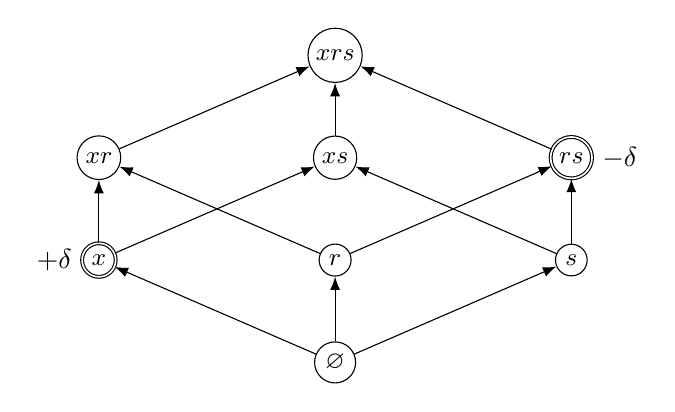
\begin{tikzpicture}[>=Latex,scale=1.0,
 v/.style={circle,draw,inner sep=2pt,font=\small},
 hot/.style={v,double},edge/.style={->,thin}]
\node[v] (o) at (0,0) {\(\varnothing\)};
\node[hot,label=left:\(+\delta\)] (x) at (-3,1.3) {\(x\)};
\node[v] (r) at (0,1.3) {\(r\)};\node[v] (s) at (3,1.3) {\(s\)};
\node[v] (xr) at (-3,2.6) {\(xr\)};
\node[v] (xs) at (0,2.6) {\(xs\)};
\node[hot,label=right:\(-\delta\)] (rs) at (3,2.6) {\(rs\)};
\node[v] (all) at (0,3.9) {\(xrs\)};
\foreach \a/\b in {o/x,o/r,o/s,x/xr,x/xs,r/xr,r/rs,s/xs,s/rs,xr/all,xs/all,rs/all}
\draw[edge] (\a)--(\b);
\end{tikzpicture}
\caption{Complementary exceptional vertices.  No maximal chain visits both.
Deleting the distinguished label leaves the difference of two smaller
path families.  Numerical equality of labels does not identify vertices.}
\label{fig:antichain}
\end{figure}

\subsection{The nested marked identity}
Fix a strict divisibility chain
\begin{equation}\label{eq:chain}
e=p_0<p_1<\cdots<p_L=P\mid d,\qquad L\ge1,
\qquad \mathcal B_{p_i}\text{ is }p_{i+1}\text{-periodic}\quad(0\le i<L).
\end{equation}
These are period hypotheses, not least-period hypotheses.  Take a positive
labeled list
\begin{equation}\label{eq:detector-list}
\mathbf a=(a,y_{L-1},\ldots,y_0,r,s,z),\qquad \sum\mathbf a=n,
\end{equation}
where \(a\in\supp v\), the target is \(t=y_{L-1}\), and
\begin{equation}\label{eq:layers}
y_i\in p_i\Z\setminus p_{i+1}\Z\quad(0\le i<L),\qquad e\nmid r,s,z.
\end{equation}
When \(L=1\), every subsequence indexed from \(0\) to \(L-2\) is empty
and \(y_0=t\).  Put
\begin{equation}\label{eq:deltaH}
\begin{split}
\Delta&=b(a+t)-b(t),\\
\theta_i&=\mathcal B_{p_{i+1}}(y_i+y_{i+1})-\mathcal B_{p_{i+1}}(y_i)\quad(0\le i\le L-2),\\
f_y(x)&=\mathcal B_e(x+y)-\mathcal B_e(x),\\
H_y(r,s,z)&=f_y(r)(w(s)+w(z))+f_y(s)(w(r)+w(z))
+f_y(z)(w(r)+w(s)).
\end{split}
\end{equation}

For a labeled list \(\mathbf M=(m_1,\ldots,m_k)\), define
\begin{equation}\label{eq:J}
\Jcal_y(\mathbf M)=\sum_{\pi\in\mathfrak S_k}\left[
\prod_{j=1}^{k-1}b\left(y+\sum_{h=1}^jm_{\pi(h)}\right)
-\prod_{j=1}^{k-1}b\left(\sum_{h=1}^jm_{\pi(h)}\right)\right].
\end{equation}

\begin{theorem}\label{thm:nested}
Under \eqref{eq:chain}--\eqref{eq:layers},
\begin{equation}\label{eq:nested-product}
\Delta K=-v(a)\Delta
\left(\prod_{i=0}^{L-2}\theta_i\right)H_{y_0}(r,s,z).
\end{equation}
The empty product is one.  The absolute value is at most two, and the list
has \(L+4\) labels.
\end{theorem}
\begin{proof}
The sum \(r+s+z\) is divisible by \(e\).  Every nonempty proper subset
of these three labels has sum off the \(e\)-grid: for two labels, its
sum is the negative of the remaining label modulo \(e\).  Adding higher
labels does not change this.  A subset containing no bottom label has a
lowest neutral layer, whose contribution cannot be canceled by higher
layers.  If all bottom labels occur, apply the same observation to the
complement.  The only proper nonempty subset sums of the full list on the
\(d\)-grid are therefore \(a\) and \(n-a\).

Their increments from \(c\) to \(b\) are \(v(a)\) and \(-v(a)\).
The antichain identity gives
\[
\Delta K=v(a)\Jcal_a(t,y_{L-2},\ldots,y_0,r,s,z).
\]
In the remaining list, only \(\{t\}\) and its complement have proper
subset sums on the \(p_{L-1}\)-grid, by the same lowest-layer argument.
At all other vertices the shift \(a\) preserves the cut value, since
\(P\mid d\mid a\) and \(\mathcal B_{p_{L-1}}\) has period \(P\).
The two exceptional increments are \(\Delta\) and
\[
b(n-t)-b(n-a-t)=b(-t)-b(-a-t)=-\Delta.
\]
Here \(t,a+t\) lie on the \(e\)-grid and off the \(d\)-grid,
where the cut values are even under reflection.  Deleting the first or
last label therefore leaves
\(v(a)\Delta\Jcal_t(y_{L-2},\ldots,y_0,r,s,z)\).

For an intermediate step \(1\le i<L\), let
\[
\mathbf M_i=(y_{i-1},\ldots,y_0,r,s,z),\qquad
T_i=\sum\mathbf M_i,\qquad A_i=T_i+y_i=n-a-\sum_{k>i}y_k.
\]
The integer \(A_i\) is divisible by \(p_{i+1}\), and the total
\(T_i\) is divisible by \(p_i\).  In \(\mathbf M_i\), the only
proper subset sums on the \(p_{i-1}\)-grid are those of
\(\{y_{i-1}\}\) and its complement.  At every other vertex, shifting
by \(y_i\) preserves the cut value because \(p_i\mid y_i\) and
\(\mathcal B_{p_{i-1}}\) has period \(p_i\).  Write \(x=y_{i-1}\).
The singleton increment is \(\theta_{i-1}\).  At the complement it is
\begin{align*}
b(T_i-x+y_i)-b(T_i-x)
&=\mathcal B_{p_i}(A_i-x)-\mathcal B_{p_i}(A_i-y_i-x)\\
&=\mathcal B_{p_i}(-x)-\mathcal B_{p_i}(-y_i-x)\\
&=\mathcal B_{p_i}(x)-\mathcal B_{p_i}(x+y_i)=-\theta_{i-1}.
\end{align*}
Both arguments in the first line are off the \(p_i\)-grid.  The second
line uses period \(p_{i+1}\), and the third uses the zero odd part at
multiples of \(e\).  If \(\mathbf R_i=(y_{i-2},\ldots,y_0,r,s,z)\),
with \(\mathbf R_1=(r,s,z)\), antichain contraction gives
\[
\Jcal_{y_i}(y_{i-1},\mathbf R_i)
=\theta_{i-1}\Jcal_{y_{i-1}}(\mathbf R_i).
\]
This explicitly removes every intermediate label and leaves
\(\Jcal_{y_0}(r,s,z)\) times the stated scalar factors.

At the bottom put \(y=y_0\).  Since \(y+r+s+z\equiv0\pmod{p_1}\),
the contribution with first label \(q_1\) and last label \(q_2\) is
\[
\mathcal B_e(y+q_1)\mathcal B_e(-q_2)-\mathcal B_e(q_1)\mathcal B_e(-y-q_2).
\]
Period \(p_1\) justifies the complementary arguments.  Using
\(\mathcal B_e(-x)=\mathcal B_e(x)-w(x)\) and \(w(y+x)=w(x)\), this becomes
\[
f_y(q_1)\mathcal B_e(q_2)-\mathcal B_e(q_1)f_y(q_2)-f_y(q_1)w(q_2).
\]
The first two terms cancel on summing over the six ordered pairs of
labels, even if numerical values coincide.  The remaining sum is
\(-H_y(r,s,z)\), proving \eqref{eq:nested-product}.

Finally, \(f_y,w\) are disjoint ternary functions: a nonzero value of
\(w\) forces the binary cut value, which is unchanged by an
\(e\)-multiple shift.  On three positions at most two mixed products
in \(H_y\) are nonzero.  Thus \(|H_y|\le2\).  Every other factor is
zero or a unit, proving the bound.
\end{proof}

\subsection{Least periods select nonzero probes}

\begin{lemma}\label{lem:bottom}
Suppose \(\mathcal B_e\) has least period \(p>e\).  If \(e\mid y\) and \(p\nmid y\), there
are \(0<r,s,z<p\), all off the \(e\)-grid, such that
\begin{equation}\label{eq:bottom-probes}
r+s+z\equiv-y\pmod p,\qquad H_y(r,s,z)\ne0.
\end{equation}
\end{lemma}
\begin{proof}
The function \(f_y=\mathcal B_e(\cdot+y)-\mathcal B_e\) on \(\Z/p\Z\) is nonzero, vanishes
on \(e\Z\), has zero sum on every \(e\)-residue class, and satisfies \(wf_y=0\).
Moreover,
\begin{equation}\label{eq:shifted-reflection}
f_y(-y-x)=-f_y(x).
\end{equation}
Suppose \(H_y(r,s,z)=0\) for every triple satisfying
\(0<r,s,z<p\), \(e\nmid r,s,z\), and
\(r+s+z\equiv-y\pmod p\).  Substituting \(z=-y-r-s\), equation
\eqref{eq:shifted-reflection} and the oddness and \(e\)-periodicity of \(w\) give
\[
w(r)f_y(s)+f_y(r)w(s)
=w(r+s)(f_y(r)+f_y(s))+f_y(r+s)(w(r)+w(s))
\]
whenever \(r,s,r+s\) are off the \(e\)-grid.  If \(r\) is on that
grid, then \(w(r)=f_y(r)=0\) and \(w(r+s)=w(s)\), so the remaining
products vanish by \(wf_y=0\).  The case of \(s\) on the grid is
identical.  If \(r+s\) is on the grid, then \(w(s)=-w(r)\); either
both \(w\)-values or both corresponding \(f_y\)-values vanish.
Thus the equation holds on the whole circle.
\Cref{lem:fiber} and the zero residue-class sums would force \(f_y=0\),
a contradiction.
\end{proof}

\begin{lemma}\label{lem:selection}
Suppose the periods in \eqref{eq:chain} are least periods, and fix
\(t\in p_{L-1}\Z\setminus P\Z\).  The probes can be chosen so that
\begin{equation}\label{eq:probe-bounds}
0<y_i<p_{i+2},\quad\theta_i\ne0\quad(0\le i\le L-2),
\qquad 0<r,s,z<p_1,\quad H_{y_0}(r,s,z)\ne0,
\end{equation}
with the layer conditions \eqref{eq:layers} and
\begin{equation}\label{eq:sum-congruence}
t+\sum_{i=0}^{L-2}y_i+r+s+z\equiv0\pmod{p_1}.
\end{equation}
\end{lemma}
\begin{proof}
Set \(y_{L-1}=t\) and work downward.  Once \(y_{i+1}\) is chosen,
translation by it is not a period of \(\mathcal B_{p_{i+1}}\), whose least period
is \(p_{i+2}\).  The nonzero difference
\[
\mathcal B_{p_{i+1}}(x+y_{i+1})-\mathcal B_{p_{i+1}}(x)
\]
vanishes on the \(p_{i+1}\)-grid.  It also vanishes off the
\(p_i\)-grid, where both mask values agree with \(\mathcal B_{p_i}\) and the
shift is a multiple of its period \(p_{i+1}\).  A nonzero value thus
occurs in \(p_i\Z\setminus p_{i+1}\Z\).  The difference has period
\(p_{i+2}\); choose a representative \(0<y_i<p_{i+2}\) there.
At the bottom \(e\mid y_0\) but \(p_1\nmid y_0\), so
\cref{lem:bottom} supplies the last three probes.  When \(L=1\), it
applies directly to \(y_0=t\).  The bottom congruence cancels \(y_0\),
and every higher probe is divisible by \(p_1\), proving
\eqref{eq:sum-congruence}.
\end{proof}

\section{Realization at the original weight}\label{sec:realization}

The list selected by \cref{lem:selection} initially has only the required
congruence.  It must be made into a positive list of total \(n\) before its
chain sum is an inventory coefficient.

\begin{lemma}\label{lem:packing}
In the least-period setting of \cref{lem:selection}, let \(0<a<n\)
represent an element of \(\supp v\), and write
\begin{equation}\label{eq:packing-ledger}
W=n-a,\quad P=p_L,\quad
\Sigma=\sum_{i=0}^{L-2}y_i+r+s+z,\quad
C_{\mathrm{box}}=3p_1+\sum_{i=2}^{L}p_i.
\end{equation}
Suppose \(0<t<W\) and \(b(a+t)\ne b(t)\).  If
\begin{equation}\label{eq:packing-budget}
W\ge C_{\mathrm{box}}-p_1,
\end{equation}
then the selected probes or their reflected versions can be padded to a
positive detector of total \(n\), without changing the nonzero product in
\eqref{eq:nested-product}.  In particular, \(W\ge2P\) suffices.
\end{lemma}
\begin{proof}
Reflect the target and probes as in \cref{fig:packing}:
\[
t'=W-t,\quad y_{L-1}'=t',\quad
y_i'=p_{i+2}-y_i\quad(0\le i\le L-2),\quad
(r',s',z')=(p_1-r,p_1-s,p_1-z).
\]
All reflected probes remain positive and in the same divisibility layers.
Their sum is \(\Sigma'=C_{\mathrm{box}}-\Sigma\).

The original list fits if \(\Sigma\le W-t\).  Otherwise the congruence
\eqref{eq:sum-congruence} forces
\[
\Sigma\ge W-t+p_1,
\qquad
\Sigma'\le C_{\mathrm{box}}-W+t-p_1\le t.
\]
So the reflected list fits.  Strict divisibility gives
\(2p_1+p_2+\cdots+p_L\le2p_L\), which proves that \(W\ge2P\) suffices.

At each intermediate level \(0\le i\le L-2\),
\(y_i'\equiv-y_i\) and \(y_{i+1}'\equiv-y_{i+1}\pmod{p_{i+2}}\).
For \(i=L-2\), the latter congruence uses \(P\mid W\); at lower levels,
it uses \(p_{i+2}\mid p_{i+3}\).
The mask \(\mathcal B_{p_{i+1}}\) has that period and is even at these multiples of
\(e\), so
\[
\theta_i'=\theta_i.
\]
At the bottom,
\(f_{-y}(-x)=f_y(x)\) because the two odd parts cancel under an
\(e\)-multiple shift, whereas \(w(-x)=-w(x)\).  Consequently
\(H_{y_0'}(r',s',z')=-H_{y_0}(r,s,z)\).
Finally, \(t,a+t\) are neutral off-\(d\)-grid positions, and
\[
\Delta':=b(a+t')-b(t')
=b(-t)-b(-a-t)
=-\bigl(b(a+t)-b(t)\bigr).
\]
The two minus signs cancel; the entire product retains its sign.

In the fitting orientation, the remaining deficit is a nonnegative
multiple of \(p_1\).  Add it to one bottom probe.  Every factor in the
product is unchanged, and the final list satisfies
\begin{equation}\label{eq:original-weight}
a+t+\sum_{i=0}^{L-2}y_i+r+s+z=n.
\end{equation}
Use the primed variables in this equation when reflection was needed.
The upper bounds in \eqref{eq:probe-bounds} apply to the initially selected
probes; the identity itself requires only positivity, the layer conditions,
and \eqref{eq:original-weight}.
\end{proof}

\begin{example}\label{ex:reflection}
Let \(n=30\), \(e=5\), and \(p_1=d=10\).  Start with the periodic mask
\[
(\mathcal B_5(0),\ldots,\mathcal B_5(9))=(0,1,1,0,0,0,1,0,1,0),
\]
and set the remaining cuts by
\[
b(5)=b(25)=1,\quad b(15)=0,\quad b(10)=1,\quad b(20)=0.
\]
Let \(c\) agree with \(b\) except at \(10,20\), where the values are
exchanged.  Take \(a=10\), \(W=20\), and \(t=15\).  The bottom probes
\((9,8,8)\) give \(H_t=2\) and \(\Delta=1\), but their sum is \(25\),
whereas \(W-t=5\).  Reflection gives target \(5\), probes \((1,2,2)\),
\(H_5=-2\), and \(\Delta'=-1\).  Padding the first probe by \(10\)
gives the positive weight-\(30\) list \((10,5,11,2,2)\).  Its labeled
difference is \(-2\), and exact division by \(2!\) gives ordinary
coefficient difference \(-1\) at \((11,10,5,2,2)\).
\end{example}

\begin{figure}[ht]
\centering
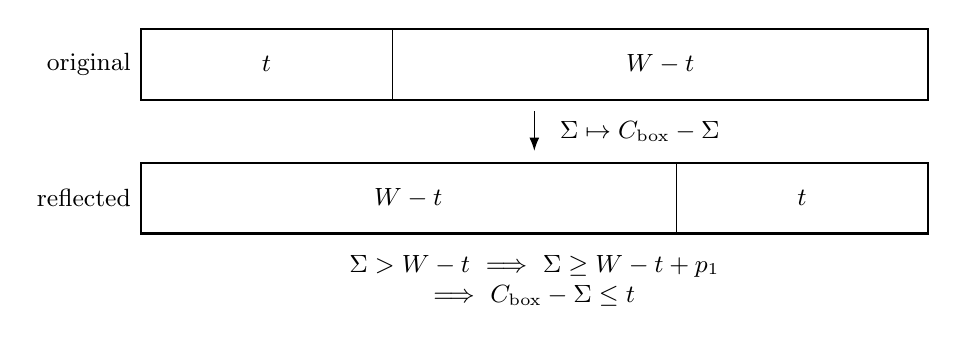
\begin{tikzpicture}[>=Latex,x=1cm,y=1cm,font=\small]
\draw[thick] (0,1.7) rectangle (10,2.6);
\draw (3.2,1.7)--(3.2,2.6);
\node at (1.6,2.15) {\(t\)};\node at (6.6,2.15) {\(W-t\)};
\node[left] at (0,2.15) {original};
\draw[thick] (0,0) rectangle (10,.9);
\draw (6.8,0)--(6.8,.9);
\node at (3.4,.45) {\(W-t\)};\node at (8.4,.45) {\(t\)};
\node[left] at (0,.45) {reflected};
\draw[->] (5,1.55)--(5,1.05);
\node[right] at (5.2,1.3) {\(\Sigma\mapsto C_{\mathrm{box}}-\Sigma\)};
\node[align=center] at (5,-.6)
{\(\Sigma>W-t\ \Longrightarrow\ \Sigma\ge W-t+p_1\)
\\\(\Longrightarrow\ C_{\mathrm{box}}-\Sigma\le t\)};
\end{tikzpicture}
\caption{The reflection changes which complementary interval accommodates
the probes.  The lattice overshoot is at least \(p_1\).  The ambient weight
remains \(a+W=n\) throughout; the drawing is schematic, not to scale.}
\label{fig:packing}
\end{figure}

\begin{proposition}\label{prop:propagation}
Suppose \eqref{eq:chain} consists of least periods.  If all applicable
positive detectors of \cref{thm:nested} vanish, then \(\mathcal B_P\) is
\(d\)-periodic.
\end{proposition}
\begin{proof}
Outside the \(p_{L-1}\)-grid, invariance under any support shift
\(a\in\supp v\) follows from period \(P\mid d\) of
\(\mathcal B_{p_{L-1}}\).  Consider
\(t\in p_{L-1}\Z\setminus P\Z\) with \(0<t<n-a\).
If \(n-a\ge2P\) and \(b(a+t)\ne b(t)\), the nonzero probes of
\cref{lem:selection} and the positive realization of \cref{lem:packing}
give a nonzero detector, contrary to the hypothesis.  Therefore
\[
b(t+a)=b(t)\qquad(0<t<n-a)
\]
whenever the indicated layer and length conditions hold.

Suppose first that \(P<d\), so \(d\ge2P\).  For every support point
\(a\), both \(a\) and \(n-a\) are positive multiples of \(d\).
Apply the nonwrapped equality to both support points.  The first handles
\(0<t<n-a\).  If \(n-a<t<n\), put \(x=t-(n-a)\); then
\(0<x<a\), and the complementary application gives
\[
b(t)=b(x+n-a)=b(x)=b(t+a),
\]
with the last argument read modulo \(n\).  The omitted endpoint
\(t=n-a\) lies on the \(P\)-grid and is not in the target layer.
Thus every support shift preserves the cut values in that layer.  The
previous mask handles positions off the \(p_{L-1}\)-grid, and
\(\mathcal B_P\) is zero on the \(P\)-grid.  Since the support generates
\(d\Z/n\Z\), the mask is \(d\)-periodic.

Now suppose \(P=d\) and \(d\in\supp v\).  Choose \(a=d\).
The budget \eqref{eq:packing-budget} holds because \(n/d\ge3\), hence \(n-d\ge2d\).
For a residue \(0<r<d\) in
\(p_{L-1}\Z\setminus d\Z\), the nonwrapped equalities join every
successive pair in
\[
r,\ r+d,\ \ldots,\ r+(n/d-1)d.
\]
All their cut values agree, so the final cyclic wrap agrees too.
Again the previous mask handles positions off the \(p_{L-1}\)-grid
and \(\mathcal B_d\) vanishes on its grid.  This proves \(d\)-periodicity.

Finally suppose \(P=d\) and \(d\notin\supp v\).  Oddness also
excludes \(n-d\).  Every support representative and its complement
are at least \(2d\), so both directional budgets are available.
The two-direction argument of the first case now applies with \(P=d\).
Every support shift preserves \(\mathcal B_d\); since those shifts generate the
\(d\)-grid, it is \(d\)-periodic.  The three cases are exhaustive.
\end{proof}

\begin{proposition}\label{prop:termination}
Assume the starting mask and every subsequent propagation succeed.
Set
\[
p_0=e,\qquad p_{j+1}=\per(\mathcal B_{p_j}).
\]
Then \(p_j\mid p_{j+1}\mid d\) at every step.  The chain stabilizes at a
proper inner size \(p\) for which, after the chosen orientation,
\begin{equation}\label{eq:common-factor}
\beta=\delta\circ\epsilon,\qquad
\gamma=\zeta\circ\epsilon,\qquad 3\le|\epsilon|=p\le d<n.
\end{equation}
\end{proposition}
\begin{proof}
Every mask obtained in the iteration is \(d\)-periodic, so its least period
divides \(d\).  Suppose the divisibilities have been proved through \(p_j\),
and let \(r\) be a period of \(\mathcal B_{p_j}\).  Its odd part is \(w\),
so \(p_0=e\mid r\).  For \(0\le k<j\), if \(p_k\mid r\), setting the
values on the \(p_k\)-grid to zero recovers \(\mathcal B_{p_k}\), since
\(p_k\mid p_j\).  Translation by \(r\) preserves that grid, so this
remasking preserves period \(r\).  Consequently
\(p_{k+1}=\per(\mathcal B_{p_k})\mid r\).  Induction on \(k\) gives
\(p_j\mid r\); when \(j=0\), the odd-part argument already suffices.
Apply this to \(r=\per(\mathcal B_{p_j})\) to obtain
\(p_j\mid p_{j+1}\mid d\), completing the induction on \(j\).

Each strict increase is followed by \cref{prop:propagation}.  A divisor
chain inside \(d\) must stabilize.  At its stable value \(p\),
\(b(x+p)=b(x)\) for \(p\nmid x\).  The two originals agree outside the
\(p\)-grid because their changed support is contained in \(d\Z\) and
\(p\mid d\).  Let \(\epsilon\) be the composition of weight \(p\) with cuts
\(S(\beta)\cap\{1,\ldots,p-1\}\), and let \(\delta,\zeta\) have cuts
\(\{x:px\in S(\beta)\}\) and \(\{x:px\in S(\gamma)\}\).
Equation \eqref{eq:composition-cuts} proves the literal factorizations
\eqref{eq:common-factor}.  The bounds follow from \eqref{eq:basic-periods}.
\end{proof}

\begin{proposition}\label{prop:local-alternative}
For two compositions of weight \(n\), either they are identical or reversed,
or, after orientation, a proper literal common inner factor is found,
or some ordinary coefficient differs by one or two.  The initial tests
use at most three blocks; failure of the starting mask uses four blocks;
failure after \(L\ge1\) strict mask increases uses \(L+4\) blocks.
In the last cases,
\begin{equation}\label{eq:coarse-local-budget}
L\le\Omega(d/e),\qquad
4+\Omega(d/e)\le\Omega(n)+2.
\end{equation}
The distinguishing partition has distinct parts except possibly one pair.
\end{proposition}
\begin{proof}
\Cref{lem:low-order} either supplies a small certificate or establishes exact
low-order identities.  Remove the identical and reversal cases, and
normalize by \cref{prop:normalization}.

If a special four-block expression in \cref{lem:four-start} is nonzero,
it has labeled magnitude at most two and gives an ordinary certificate
by \cref{lem:labels}.  Otherwise the first mask is \(d\)-periodic.
At a subsequent defect, \cref{lem:selection,lem:packing,thm:nested}
supply an original-weight nonzero detector of labeled magnitude at most
two.  If no defect occurs, \cref{prop:termination} supplies the factor.

A strict period increase consumes at least one prime factor of \(d/e\).
Since \(e\ge3\) and \(n/d\ge3\),
\[
4+\Omega(d/e)=\Omega(n)+4-\Omega(e)-\Omega(n/d)
\le\Omega(n)+2.
\]
The repeated-part assertion follows from \cref{lem:labels}.
No full-inventory equality was used to obtain this alternative: only
vanishing of the explicitly tested bounded discrepancies was used.
\end{proof}

\section{Recognition by descent and composition congruence}\label{sec:recognition}

\begin{theorem}[Coarse recognition]\label{thm:coarse}
For compositions \(\beta,\gamma\) of weight \(n\), either they have a
factor-reversal witness and \(\Psi_\beta=\Psi_\gamma\), or some
\(\lambda\vdash n\) satisfies
\begin{equation}\label{eq:coarse-certificate}
\ell(\lambda)\le\Omega(n)+2,
\qquad m_\beta(\lambda)-m_\gamma(\lambda)\in\{-2,-1,1,2\}.
\end{equation}
The alternatives are exclusive.  The certificate may have distinct parts
except possibly one repeated pair.
\end{theorem}
\begin{proof}
Use strong induction on \(n\), with both the witness and equality of the
whole substitution maps as the successful output.
Literal equality and reversal give this output directly by
\cref{prop:unsigned}.  In every other case, \cref{prop:local-alternative}
either supplies \eqref{eq:coarse-certificate} or gives
\[
\beta=\delta\circ\epsilon,\qquad
\eta=\zeta\circ\epsilon,\qquad
\eta\in\{\gamma,\gamma^*\},\qquad p=|\epsilon|>1.
\]
Apply the induction hypothesis to the outer pair of weight \(n/p\).
For any partition \(\mu\vdash n/p\), retaining only grid cuts gives
\begin{equation}\label{eq:coefficient-grid}
m_\beta(p\mu)=m_\delta(\mu),\qquad
m_\eta(p\mu)=m_\zeta(\mu).
\end{equation}
Thus an outer certificate lifts unchanged in magnitude and number of
blocks, and \(\Omega(n/p)+2\le\Omega(n)+2\).

Otherwise induction gives \(\Psi_\delta=\Psi_\zeta\) and a factor witness.
Compose the maps on the left with \(\Psi_\epsilon\) and use
\eqref{eq:Psi-laws}.  Append \(\epsilon\) to the witness.  If
\(\eta=\gamma^*\), reverse every factor on the second side, using
\((\alpha\circ\epsilon)^*=\alpha^*\circ\epsilon^*\); the order of the
factor list is not reversed.  This gives the desired witness and map
equality for the original pair.

A factor witness preserves the complete inventory by
\cref{cor:reversal-suffices}, so the alternatives are exclusive.
Scaling in \eqref{eq:coefficient-grid} preserves repeated-part
multiplicities.
\end{proof}

\begin{remark}\label{rem:shallow-induction}
The outer pair is not assumed fully equivalent at extraction.  It receives
the induction alternative.  In a formulation starting from shallow
congruence, \eqref{eq:coefficient-grid} transfers that shallow congruence,
and the smaller-weight theorem then gives full equality.
\end{remark}

\begin{proposition}\label{prop:budget}
Let \(H:\N\to\N\) be monotone under divisibility.  Suppose it covers the
initial low-order tests and every applicable local detector in
\cref{prop:local-alternative}: three blocks for \(n\ge5\), two blocks for
\(2\le n\le4\), four blocks whenever the starting mask requires a test,
and \(L+4\) after \(L\ge1\) strict mask increases requiring a detector.
Then \cref{thm:coarse} holds with \(H(n)\) in place of
\(\Omega(n)+2\).
\end{proposition}
\begin{proof}
Repeat the same induction, using \(H(n/p)\le H(n)\) in
\eqref{eq:coefficient-grid}.  At weights at most four, two-block data
fix every symmetric cut pair and the midpoint, with at most one
asymmetric reflected pair left; its two orientations are global reversals.
Weight one has a single composition.  The other local costs are exactly
the stated detector costs.
\end{proof}

\begin{proof}[Proof of \cref{thm:main-structure}]
If inventories are equal, the certificate alternative in
\cref{thm:coarse} is impossible.  Conversely, equality of the maps gives
equality on \(h_1\), and a factor witness preserves \(G\).
If
\(\alpha\sim\alpha'\) and \(\beta\sim\beta'\), then
\begin{equation}\label{eq:congruence}
\alpha\circ\beta\sim\alpha'\circ\beta'.
\end{equation}
For \eqref{eq:congruence}, use
\(\Psi_{\alpha\circ\beta}=\Psi_\beta\Psi_\alpha\).
Equality on all generators gives every near-power simultaneously.
\end{proof}

Thus composition descends to the equivalence classes.  The class of
\(\epsilon\) determines \(\Psi_\epsilon\), and equality of these maps
reflects equality of classes by evaluation at \(h_1\).  The composition
law reverses the order of the corresponding endomorphisms.  For a fixed
right factor, the grid left inverse also reflects equivalence of the outer
factors; no choice of a representative of an inner class is required.

\begin{corollary}\label{cor:class}
For every \(m\ge1\),
\[
\Ec((m)\circ\beta)
=\{(m)\circ\gamma:\gamma\in\Ec(\beta)\}.
\]
\end{corollary}
\begin{proof}
The inclusion from right to left is \eqref{eq:REV}.
For the reverse inclusion, use strong induction on \(N=mn\), where
\(n=|\beta|\).  Put \(F=\beta^{\odot m}\), and suppose \(\eta\sim F\).
If \(\eta=F\) or \(F^*\), take \(\gamma=\beta\) or \(\beta^*\).
Otherwise \cref{prop:local-alternative}, with its certificate excluded
by inventory equality, gives
\[
F=\alpha\circ\epsilon,\qquad
\eta'=\zeta\circ\epsilon,\qquad
\eta'\in\{\eta,\eta^*\},\qquad
1<p=|\epsilon|<N.
\]
By \eqref{eq:split}, \(G_\alpha=G_\zeta\).

Suppose first that \(p\nmid n\).  Let \(B\) be the cyclic cut indicator
of \(F\) on \(\Z/N\Z\).  It is \(n\)-periodic, and its values off the
\(p\)-grid depend only on the residue modulo \(p\).
If \(j\in S(\alpha)\), then \(B(pj)=B(pj+n)=1\).
Since \(pj+n\) and \(n\) are off the \(p\)-grid and congruent modulo
\(p\), this gives \(B(n)=1\), contrary to the absence of near-power
seam cuts.  Thus \(\alpha=(N/p)\).
Its inventory has ordinary degree one, so \(G_\zeta=G_\alpha\)
forces \(\zeta=\alpha\).  Hence \(\eta'=F\), and the conclusion follows.

Now suppose \(p\mid n\), and put \(k=n/p\).
Restricting the cut formula to the first \(n\)-cell and applying
\cref{lem:literal-factor} gives \(\beta=\delta\circ\epsilon\).
Equation \eqref{eq:composition-cuts} and uniqueness at inner weight
\(p\) then give \(\alpha=\delta^{\odot m}\).
Since \(mk=N/p<N\), the induction hypothesis applied to
\(\zeta\sim\delta^{\odot m}\) gives
\[
\zeta=\xi^{\odot m},\qquad \xi\sim\delta.
\]
Set \(\gamma=\xi\circ\epsilon\).
By \eqref{eq:substitution}, \(\gamma\sim\beta\), and the cut formula gives
\(\eta'=\gamma^{\odot m}\).
If \(\eta'=\eta^*\), replace \(\gamma\) by \(\gamma^*\).
Literal reversal preserves \(G\) and commutes with near-powers.
\end{proof}

\begin{corollary}\label{cor:modular-budget}
Under a budget \(H\) in \cref{prop:budget}, ordinary inventory coefficients
through \(H(n)\) modulo any integer \(q\ge3\) determine the complete inventory.
\end{corollary}
\begin{proof}
A nonzero discrepancy of magnitude one or two is nonzero modulo \(q\).
Apply the exact integer alternative.  No labeled factorial is inverted
modulo \(q\).
\end{proof}

\section{Arithmetic bounds and sharp cumulative depth}\label{sec:depth}

\subsection{Restrictions on period growth}
\begin{lemma}\label{lem:ratios}
In the normalized mask argument:
\begin{enumerate}
\item if \(e=3\), a common inner factor of weight three is immediate;
\item if \(e=4\), the first strict mask period cannot be eight;
\item a strict chain of successive least mask periods cannot contain \(p,2p,4p\) consecutively.
\end{enumerate}
\end{lemma}
\begin{proof}
For \(e=3\), the nonzero odd ternary function \(w\) is nonzero on both
nonzero residue classes.  The corresponding binary cut values are forced:
\(b=1\) where \(w=1\) and \(b=0\) where \(w=-1\).  They agree for the originals
and repeat modulo three.  The cuts on the three-grid are arbitrary outer
cuts, giving the common inner factor without a four-block test.

For \(e=4\), a nonzero odd function of period four is nonzero on the odd
residues and zero on residue two.  If \(\mathcal B_4\) had least period eight, its
values at \(1,5\) and at \(3,7\) would agree by the forced odd bits.  Its
values at \(2,6\) agree by evenness at those neutral positions; it is zero
at \(0,4\).  It would therefore already be four-periodic.

Suppose \(\mathcal B_p\) has period \(2p\) and \(\mathcal B_{2p}\) has least period \(4p\).
Off the \(p\)-grid, \(\mathcal B_{2p}=\mathcal B_p\), so it is \(2p\)-periodic there.
On the \(p\)-grid modulo \(4p\), the values at \(0,2p\) are zero, and those at
\(p,3p\) agree by \eqref{eq:mask-odd}, since \(e\mid p\).  Thus \(\mathcal B_{2p}\) is
\(2p\)-periodic everywhere, a contradiction.
\end{proof}

For integers \(e\ge4\) and \(D\ge1\), let \(a_2=\nu_2(D)\) be the
exponent of \(2\) in \(D\), and put \(a_o=\Omega(D)-a_2\).  Define
\begin{equation}\label{eq:T}
\varepsilon_e=\begin{cases}0,&e=4,\\1,&e\ge5,\end{cases}
\qquad
T_e(D)=\min\left\{a_2+a_o,
\left\lfloor\frac{2a_2+4a_o+\varepsilon_e}{3}\right\rfloor\right\}.
\end{equation}
\begin{lemma}\label{lem:arithmetic-optimization}
Let \(e\ge4\), \(D\ge1\), \(a_2=\nu_2(D)\) and \(a_o=\Omega(D)-a_2\).
The largest length of a list of integers at least two whose product
divides \(D\), with no adjacent entries equal to two and with the first
entry different from two when \(e=4\), is \(T_e(D)\) in \eqref{eq:T}.
\end{lemma}
\begin{proof}
Write \(b=a_o\) and \(\varepsilon=\varepsilon_e\).
If \(k\) entries equal two and \(q_0\) entries are different from two, then
\[
k\le q_0+\varepsilon.
\]
If \(t_0\) of the latter entries have no odd prime factor, they use at least
two factors of two each.  Thus
\[
a_2\ge k+2t_0,\qquad b\ge q_0-t_0,
\]
and
\[
2a_2+4b\ge2k+4q_0\ge3(k+q_0)-\varepsilon.
\]
Also \(k+q_0\le a_2+b\).  These prove the two upper bounds in \eqref{eq:T}.

For attainability, treat the odd primes with multiplicity as separate
non-two entries.  If \(a_2\le b+\varepsilon\), all primes may remain separate
and the singleton twos can be interspersed in the permitted slots; this
attains \(a_2+b\).

Suppose \(a_2>b+\varepsilon\) and write
\(a_2-b-\varepsilon=3t_0+r\), \(r\in\{0,1,2\}\).
If \(r=0\) or \(1\), use \(t_0\) entries equal to four, the \(b\) odd primes,
and \(b+t_0+\varepsilon\) singleton twos.  At most one factor of two is
unused.  The resulting length is \(2b+2t_0+\varepsilon\), as required.
If \(r=2\), use \(t_0+1\) fours, the \(b\) odd primes, and
\(b+t_0+\varepsilon\) singleton twos.  This has the required length one
larger.  In either case the twos can be placed in nonadjacent slots,
with no initial two when \(\varepsilon=0\).
The product is allowed to divide \(D\), so unused prime factors cause no
problem.  The empty list covers the zero-length cases.
\end{proof}

\Cref{lem:arithmetic-optimization} proves that \(T_e(D)\) is the largest
length of a numerical list of ratios whose product divides \(D\), with no
consecutive ratios equal to two and with the first ratio different from
two when \(e=4\).  This numerical optimization is separate from any assertion
about attaining a recognition bound at a particular weight.

\begin{definition}\label{def:arithmetic-bound}
Set \(B(1)=1\) and \(B(2)=B(3)=B(4)=2\).
For \(n\ge5\), define
\begin{equation}\label{eq:arithmetic-bound}
B(n)=\min\left\{n,\
\max\left(\{3\}\cup
\{4+T_e(d/e):e\mid d\mid n,\ e\ge4,\ n/d\ge3\}\right)\right\}.
\end{equation}
An empty set of divisor candidates contributes nothing to the maximum.
\end{definition}

\begin{proposition}\label{prop:refined-budget}
The function \(B\) is monotone under divisibility and covers every
applicable detector.  For every \(n\),
\(B(n)\le\Omega(n)+2\).
Consequently the discrepancy and modular conclusions of
\cref{thm:main-recognition} hold.
\end{proposition}
\begin{proof}
An actual chain with \(L\) strict steps has ratio product dividing \(d/e\)
and obeys \cref{lem:ratios}.  Thus \(L\le T_e(d/e)\), and the required
\(L+4\) blocks are covered by \eqref{eq:arithmetic-bound}.
The starting four-block test is the case \(L=0\).  The \(e=3\) case is
immediate; the low-order tests and the elementary weights at most four
are explicitly covered.  No coarsening uses more than \(n\) blocks, so the
outer minimum by \(n\) is harmless.

If \(m\mid n\), every divisor candidate \(e\mid d\mid m\) is also a candidate
for \(n\).  Both entries in the outer minimum are nondecreasing under
this passage, and the small-weight normalizations preserve monotonicity.
Finally, \(T_e(d/e)\le\Omega(d/e)\), so
\eqref{eq:coarse-local-budget} gives the coarse upper bound.
Apply \cref{prop:budget,cor:modular-budget}.
\end{proof}

Some resulting formulas, with the normalization in
\cref{def:arithmetic-bound}, are
\begin{align*}
B(2^a)&=4+\left\lfloor\frac{2(a-4)}3\right\rfloor
&& (a\ge4),\\
B(3^a)&=a+1&&(a\ge2),\\
B(p^a)&=a+2&&(p\ge5\text{ prime},\ a\ge1).
\end{align*}
For powers of two, \(e\) and \(n/d\) each consume at least two prime
factors; the remaining ratio count obeys the nonadjacent-two restriction.
For powers of three, \(e\) consumes at least two factors and \(n/d\)
at least one.  For \(p\ge5\), each
consumes one.  These formulas concern sufficient arithmetic cutoffs,
not proved exact values of \(D_{=}\) at every prime power.

\subsection{The weight-only upper bound}
Let \(U(n)\) denote the right-hand side of \eqref{eq:frontier}, without
assuming the asserted equality with \(C(n)\).

\begin{proposition}\label{prop:logarithmic-cutoff}
For \(n\ge2\), one has \(B(n)\le U(n)\).  For every \(n\ge1\),
\[
B(n)\le2\log_6 n+\log_6 9.
\]
The additive constant cannot be decreased uniformly over all positive weights.
\end{proposition}
\begin{proof}
Fix \(n\ge5\) and a divisor candidate \(e\mid d\mid n\) in
\eqref{eq:arithmetic-bound}, and put \(L=T_e(d/e)\).
By \cref{lem:arithmetic-optimization}, there is a list
\(r_1,\ldots,r_L\ge2\) whose product divides \(d/e\), with no consecutive
twos and with the first entry different from two when \(e=4\).
Thus
\[
n=\frac nd\,e\,\frac de\ge3e\prod_{i=1}^L r_i.
\]
If \(L=2j\), at least \(j\) ratios are at least three, so their product
is at least \(6^j\).  Since \(e\ge4\),
\begin{equation}\label{eq:even-threshold}
n\ge12\cdot6^j.
\end{equation}
If \(L=2j+1\) and \(e=4\), the first ratio is not two, so the product is at
least \(3\cdot6^j\), giving \(n\ge36\cdot6^j\).  For \(e\ge5\), its minimum
is \(2\cdot6^j\), giving the sharper possible threshold
\begin{equation}\label{eq:odd-threshold}
n\ge30\cdot6^j.
\end{equation}
These inequalities include \(L=0\), where the first threshold is twelve.
They imply \(4+T_e(d/e)\le U(n)\) for every divisor candidate.
The default value three is also at most \(U(n)\) for \(n\ge5\), and the
outer minimum in \eqref{eq:arithmetic-bound} can only lower the result.
Hence \(B(n)\le U(n)\).  For \(2\le n\le4\), both values equal two.

For the logarithmic estimate, the same thresholds give
\[
\frac{6^{L+4}}{n^2}\le
\begin{cases}
9,&L=2j,\\
216/25<9,&L=2j+1.
\end{cases}
\]
The default value three satisfies \(6^3/n^2\le216/25<9\) for \(n\ge5\).
Taking the maximum over the candidates, then the outer minimum, proves
\(6^{B(n)}\le9n^2\).  The prescribed values at \(n\le4\) satisfy the
same inequality.  Taking logarithms gives the asserted bound, with
equality at \(n=2\), proving optimality of the uniform additive constant.
\end{proof}

By \cref{prop:refined-budget,prop:logarithmic-cutoff}, every unequal pair
of weight \(n\ge2\) has a distinguishing coefficient through degree
\(B(n)\le U(n)\).  Since \(U\) is nondecreasing, this gives
\(C(N)\le U(N)\); at weight one the maximum is empty.
Thus \(U\) is a sufficient weight-only cutoff.  Its noninitial transitions
are \(12,30,72,180,432,1080,\ldots\), and its explicit formula gives
\(U(n)=2\log_6 n+O(1)\).
Sharpness requires actual unequal compositions, not just numerical ratio lists.

\subsection{A lift with an all-odd induction invariant}
For compositions \(R,S\) of common weight \(w\), let
\[
\Alt_j(R,S)=R\odot S\odot R\odot\cdots\odot S\odot R
\]
have \(2j+1\) factors.  Define
\begin{equation}\label{eq:OA}
\OA_s(R,S):\quad
\text{for every }j\ge0,\quad
\bigl(G_{\Alt_j(R,S)}-G_{\Alt_j(S,R)}\bigr)^{[<s]}=0.
\end{equation}
The quantifier over every odd length is essential.  The assertion for
\(j=0\) alone would not control the odd segments produced in the next lift.

Set
\begin{equation}\label{eq:sharpness-lift}
E=R\odot S,\qquad F=R\cdot S,\qquad
R'=E\cdot(F\odot E),\qquad
S'=(E\odot F)\cdot E.
\end{equation}
Both new roots have weight \(6w\).

\begin{theorem}\label{thm:lift}
For \(s\ge2\),
\begin{equation}\label{eq:OA-lift}
\OA_s(R,S)\Longrightarrow\OA_{s+2}(R',S').
\end{equation}
Moreover,
\begin{equation}\label{eq:lift-extraction}
\partial_{h_{2w}}\partial_{h_{3w}}(G_{R'}-G_{S'})=G_R-G_S.
\end{equation}
If moreover \(\OA_s(R,S)\) holds and \(G_R-G_S\) first differs in degree
\(s\), with an ordinary unit witness at \(\lambda\vdash w\), then
\(G_{R'}-G_{S'}\) first differs in degree \(s+2\) and has the same unit
witness at \(\sort(\lambda\cup\{2w,3w\})\).
\end{theorem}
\begin{proof}
Each lifted factor consists of the six old cells
\(R,S,R,S,R,S\).  Its available cell boundaries are \(\{2,3\}\) for \(R'\)
and \(\{3,4\}\) for \(S'\).  In a near-concatenation of an odd number of alternating lifted factors,
boundaries between lifted factors are absent.  Reflection through the
midpoint exchanges the two available boundary patterns: reflection
preserves the parity of the lifted-factor index and exchanges local
boundaries two and four.

Group coarsenings by the old cell-boundary cuts retained.  Once these
cuts are chosen, every segment is an alternating near-concatenation of old cells,
and its internal coarsening inventory is an independent factor.
If only common odd boundaries are retained, the same retained subset
occurs on both sides and gives literally the same product.
If only even boundaries are retained, every segment has an even number
of cells.  Reflection reverses the order of the segments and preserves
the alternating word in each such segment.

If both parities occur, at least two cuts are retained, giving at least
three nonempty segments.  Reflection preserves each even-cell segment and
exchanges the two orientations of each odd-cell segment.  The hypothesis
\eqref{eq:OA} applies to every odd segment, whatever its length.  In the
telescoping identity for the corresponding segment inventories \(P_i,Q_i\),
\[
\prod_{i=1}^tP_i-\prod_{i=1}^tQ_i
=\sum_{j=1}^t(P_j-Q_j)
\prod_{i<j}P_i\prod_{i>j}Q_i,
\]
each nonzero summand has one difference starting in degree at least \(s\)
and \(t-1\) nonempty factors starting in degree at least one.
Since \(t\ge3\), it starts in degree at least \(s+2\).
This proves \eqref{eq:OA-lift} for every odd
number of lifted factors.  No composition compatibility theorem is used.

Expanding the two alternative seams gives
\begin{equation}\label{eq:lift-difference}
G_{R'}-G_{S'}
=G_E\left(G_R G_{S\odot R\odot S}
-G_{R\odot S\odot R}G_S\right).
\end{equation}
A composition of weight \(t\) has the term \(h_t\) once and no other term
containing \(h_t\).  Since \(|E|=2w\), the \(h_{3w}\) derivative of
\eqref{eq:lift-difference} is \(G_E(G_R-G_S)\).  The \(h_{2w}\) derivative
is therefore \eqref{eq:lift-extraction}.

Every part of \(\lambda\) is at most \(w\).  The added parts \(2w,3w\) are
distinct, exceed all old parts, and each occurs once.  Thus the derivative
transports the ordinary coefficient unchanged, with no factorial
conversion.  The low-degree vanishing and the surviving unit witness
prove the final assertion.
\end{proof}

\begin{proof}[Proof of \cref{thm:main-depth}]
For the even family, start with \(R_0=(1,1)\) and \(S_0=(2)\).
Their difference is \(h_1^2\).  Every nonempty composition of a specified
weight has the same one-block term, so \(\OA_2(R_0,S_0)\) holds at every
odd alternating length.  At each iteration, \eqref{eq:OA-lift} supplies
the all-odd hypothesis for the next pair before the exact-degree clause
of \cref{thm:lift} is applied.  After \(r\) lifts, the weight is
\(2\cdot6^r\) and the first discrepancy is \(2r+2\), with a unit witness.
For \(r=j+1\), these attain \eqref{eq:even-threshold}.

For the odd family, start with \(R_0=(1,1,3)\) and \(S_0=(1,2,2)\).
Their difference is \(h_1^2h_3-h_1h_2^2\).
They have identical two-block data.  In a near-concatenation of an odd number of
equal-weight alternating cells, reflection preserves the parity of the
cell index.  A two-block count therefore reduces to the sum of the
reflected cut bits within a single root, which is equal for these seeds;
seams are absent on both sides.  Thus \(\OA_3(R_0,S_0)\) holds for every
odd length.  Iterating \eqref{eq:OA-lift} supplies \(\OA_{3+2r}\) for
each pair after \(r\) lifts.  The exact-degree clause of \cref{thm:lift}
therefore gives weight \(5\cdot6^r\) and first discrepancy \(2r+3\),
again with a unit witness.  For \(r=j+1\), these attain
\eqref{eq:odd-threshold}.

The initial witnesses are \((1,1)\) and \((3,1,1)\), respectively.  At every
lift append the parts \(2w,3w\).  These give pairs at each transition with
no lower-degree discrepancy and a discrepancy of \(+1\) at the transition.
Combining with the upper bounds proves \eqref{eq:frontier}, including
\(N=1\) and the elementary initial intervals.  Unit witnesses remain nonzero
modulo every \(q\ge3\), proving the modular sharpness statement as well.
The comparison in \cref{prop:logarithmic-cutoff} now also gives
\(B(n)\le C(n)\) for \(n\ge2\).
\end{proof}

\begin{remark}\label{rem:exact-scope}
The exact theorem concerns \(C(N)\), not \(D_{=}(n)\) at every weight.
Equality \(D_{=}(n)=B(n)\) is not asserted.  The depth theorem is stated for
unsigned inventories.  In a direct statement about signed ribbon
\(h\)-coefficients, the coefficient of \(h_n\) first records the parity of the
composition length.  For example, the unsigned pair \((1,1),(2)\) first
differs in degree two, whereas their signed ribbon difference already has
an \(h_2\) term.  The lifted threshold pairs have equal lengths, so that
small endpoint issue does not affect the threshold families.
\end{remark}

\section{Composition coordinates and effective certificates}\label{sec:recovery}

\subsection{Integral coordinates}
\begin{proposition}\label{prop:coordinates}
Fix \(\epsilon\) of weight \(p\).  Define
\[
\Theta_\epsilon(h_r)=
\begin{cases}
G_{\epsilon^{\odot(r/p)}},&p\mid r,\\
h_r,&p\nmid r.
\end{cases}
\]
Then \(\Theta_\epsilon\) is a weight-preserving automorphism of
\(\Lambda_\Z\).  In particular,
\begin{equation}\label{eq:coordinates}
\Lambda_\Z=
\Z\bigl[G_{\epsilon},G_{\epsilon^{\odot2}},\ldots,
 h_r\ (p\nmid r)\bigr]
\end{equation}
is a polynomial ring in the displayed algebraically independent generators.
The map \(\Psi_\epsilon\pi_p\) is an idempotent retraction onto
\(\operatorname{im}\Psi_\epsilon\).
\end{proposition}
\begin{proof}
For each \(j\),
\[
G_{\epsilon^{\odot j}}=h_{pj}+R_j(h_1,\ldots,h_{pj-1}).
\]
Every term other than the one-block term has all indices smaller than \(pj\).
Thus \(\Theta_\epsilon\) is unitriangular in the ordered variables, with
an integral inverse constructed recursively.  This proves
\eqref{eq:coordinates}.  The retraction assertion follows from
\(\pi_p\Psi_\epsilon=\mathrm{id}\).
\end{proof}

\begin{proposition}\label{prop:depth-cancel}
For a nonzero polynomial \(F\) whose first ordinary degree is \(r\),
\begin{equation}\label{eq:leading-substitution}
(\Psi_\epsilon F)^{[r]}=F^{[r]}(h_j\mapsto h_{pj}).
\end{equation}
Thus fixed-inner composition preserves first distinguishing degree over
any commutative coefficient ring.  Over \(\Z\), it also preserves the gcd
of all coefficients.
\end{proposition}
\begin{proof}
Each generator image is \(h_{pj}\) plus terms of ordinary degree at least
two, proving \eqref{eq:leading-substitution}.  Relabeling the independent
variables is injective over any coefficient ring.  Integrality gives
\(\content(F)\mid\content(\Psi_\epsilon F)\), while the integral left
inverse gives the reverse divisibility.
\end{proof}

\subsection{Recovery at prescribed factor weights}
For a composition \(F\), let \(P_F\) be the sum of \(G\) over all proper prefixes,
including the empty prefix, and let \(Q_F\) be the analogous suffix sum.
For \(1\le j\le|F|\), distinguishing a block of size \(j\) gives
\[
\partial_{h_j}G_F=[P_FQ_F]_{\wt=|F|-j}.
\]
The two exterior pieces are disjoint at this weight, so they can be
coarsened independently.

\begin{theorem}\label{thm:recovery}
Let \(|\alpha|=m\) and \(|\beta|=n\).  Then
\begin{align}
\pi_n(G_{\alpha\circ\beta})&=G_\alpha,
\label{eq:outer-recovery}\\
\partial_{h_{(m-1)n+j}}G_{\alpha\circ\beta}
&=\partial_{h_j}G_\beta\qquad(1\le j\le n).
\label{eq:inner-derivative}
\end{align}
Consequently the rational-linear operator
\begin{equation}\label{eq:inner-recovery}
\mathcal L_{m,n}=\frac1n\sum_{j=1}^n
j h_j\partial_{h_{(m-1)n+j}}
\end{equation}
satisfies \(\mathcal L_{m,n}(G_{\alpha\circ\beta})=G_\beta\).
For displayed products with the same two factor weights,
\begin{equation}\label{eq:two-factor-cancel}
\alpha\circ\beta\sim\alpha'\circ\beta'
\quad\Longleftrightarrow\quad
\alpha\sim\alpha'\text{ and }\beta\sim\beta'.
\end{equation}
\end{theorem}
\begin{proof}
The outer recovery is the split substitution identity.  For the derivative
identity, first suppose \(m\ge2\).  Differentiation marks one coarsened
block of length \((m-1)n+j\) and removes its variable.  Its exterior
weight is \(n-j<n\).  If its left endpoint is \(x\), then
\(0\le x\le n-j\), and its right endpoint is
\(x+(m-1)n+j\), in the final \(n\)-cell or at the total endpoint.
The literal cut formula identifies the allowed cuts before it with the
prefix cuts of \(\beta\) up to \(x\), and the allowed cuts after it
with the suffix cuts after \(x+j\), translated by \((m-1)n\).
Deleting the central length \((m-1)n\) therefore gives a marked
\(j\)-block in a coarsening of \(\beta\), preserving every exterior
block.  Conversely, insert that length into any marked \(j\)-block.
These operations are inverse and preserve the monomial in the unmarked
blocks.  Repeated blocks are counted with their marked multiplicity,
exactly as in differentiation.  This proves \eqref{eq:inner-derivative}.
For \(m=1\), the outer composition is \((1)\), and the identity is
literal.

Weighted Euler gives
\(\sum_{j=1}^n jh_j\partial_{h_j}G_\beta=nG_\beta\).
Substitute \eqref{eq:inner-derivative} and divide by \(n\) over \(\Q\)
to obtain \eqref{eq:inner-recovery}.  The two recovery operators prove
the forward implication of \eqref{eq:two-factor-cancel}; its reverse is
\eqref{eq:congruence}.
\end{proof}

These operators recover inventories of the factors at prescribed weights.
They neither discover a factorization nor recover unique literal factor
words.  The division by \(n\) in \eqref{eq:inner-recovery} is over \(\Q\);
no such division is asserted over an arbitrary coefficient ring.  The
integral derivative identities themselves need no division.

\subsection{Checking a short certificate}
Let \(t_1,\ldots,t_s\) be the distinct part values of a partition
\(\lambda\vdash n\), with multiplicities \(\nu_1,\ldots,\nu_s\),
and let \(r=\ell(\lambda)\).  For a state
\(a=(a_1,\ldots,a_s)\), \(0\le a_i\le\nu_i\), put
\(s(a)=\sum_i a_it_i\).  Write \(\nu=(\nu_1,\ldots,\nu_s)\),
and let \(e_i\) be the \(i\)th coordinate vector.  Define \(D(0)=1\)
and, for \(a\ne0\),
\[
D(a)=\eta_b(a)\sum_{i:a_i>0}D(a-e_i),\qquad
\eta_b(a)=\begin{cases}1,&a=\nu,\\ b(s(a)),&a\ne\nu.\end{cases}
\]
Then
\begin{equation}\label{eq:subset-dp}
m_\beta(\lambda)=D(\nu).
\end{equation}
Indeed, partition the distinct orders of the selected multiset according
to their last part value.  Each predecessor contributes once, since equal
occurrences are not separately labeled.  The cut test enforces the final
partial sum except at the full state, where that sum is the endpoint \(n\).
Induction over the number of selected parts proves the recurrence.

There are \(\prod_i(\nu_i+1)\le2^r\) states and at most \(r\) terms
per state, so the count takes \(O(r2^r)\) arithmetic operations and
\(O(2^r)\) integer storage after the cut array is available.  Since the
recurrence uses only addition and binary cut tests, it also computes the
ordinary coefficient directly modulo any integer, without division.
The labeled alternative counts \(K_b\) on subsets of \(r\) labels;
that version requires exact division by \(\kappa(\lambda)\) before
modular reduction.  A certificate of \cref{thm:main-recognition} is thus
checked on its short block list rather than by expanding all coarsenings
of the original composition.

\subsection{A cut-array recognition algorithm}
The following deterministic procedure avoids expanding inventories.
At each stage the two compositions have the same weight.
\begin{enumerate}
\item If their cut words are equal or reflected, accept and record that
literal operation.
\item For both orientations of the second word, test divisors \(p\) of the
current weight for a literal common inner factor: both words must be
\(p\)-periodic off \(p\Z\) and agree there.
\item If neither orientation has a common factor of weight \(p>1\), reject.
Otherwise choose the largest available \(p\), remove that common factor,
and continue with the outer pair on the \(p\)-grid.
\end{enumerate}
Every removal is safe by the split embedding \eqref{eq:split}.
Completeness follows from the factor alternative: an equivalent pair
which is neither identical nor reversed has a proper common inner factor
in one orientation.  Reversals and removed factors reconstruct the witness
on acceptance.

On an expanded \(n\)-entry cut array, testing one divisor takes \(O(n)\)
operations.  At recursive weights \(n_i\), one has \(n_{i+1}\le n_i/2\) and
\(\sigma_0(n_i)\le\sigma_0(n)\), where
\(\sigma_0(n)\) is the number of positive divisors of \(n\).  Hence total time is
\[
O\left(\sum_i n_i\sigma_0(n_i)\right)=O(n\sigma_0(n)).
\]
This is an arithmetic-operation bound in the expanded cut-array model.
It is not a polynomial bound in the binary encoding length of large
composition parts.  Certificate checking via \eqref{eq:subset-dp} uses
ordinary counts, either integrally or directly modulo three.

\subsection{The characteristic-two boundary}\label{subsec:parity}

\begin{proposition}\label{prop:parity}
Let
\[
U_{17}=(1,1,1,1,1,1,1,1,9),\qquad
V_{17}=(1,1,2,4,2,1,1,2,3).
\]
Then
\[
G_{U_{17}}^{[\le3]}\equiv G_{V_{17}}^{[\le3]}\pmod2,
\qquad G_{U_{17}}\ne G_{V_{17}}.
\]
Specifically, the coefficients at \((14,2,1)\) are two and zero,
while those at \((14,1,1,1)\) are one and zero.
\end{proposition}
\begin{proof}
Both cut sets contain exactly one point of every reflected pair modulo
17.  They are
\[
\{1,2,3,4,5,6,7,8\},\qquad
\{1,2,4,8,10,11,12,14\}.
\]
Their disagreement set is
\(\{3,5,6,7,10,11,12,14\}\), a complete doubling-negation orbit modulo 17.

For any odd weight and cut indicator with \(b(x)+b(-x)=1\) off zero,
a three-part partition with distinct parts and \(k\) cut bits equal to one
has ordinary multiplicity \(k(3-k)\in\{0,2\}\).  Indeed, an order contributes
\(b(\text{first})(1-b(\text{last}))\).
For a repeated partition \((a,a,n-2a)\), its coefficient is one precisely
when \(b(a)=b(2a)\), and zero otherwise.  This follows by writing its three
possible numerical orders; the middle order contributes
\(b(a)b(n-a)=0\).  If all three parts coincide, both descriptions give zero.
Thus two such indicators have equal three-block data modulo two exactly
when their disagreement bits are constant on doubling orbits.  Their
one- and two-block data already agree.  This proves the congruence.

For \(U_{17}\), the ordered coarsenings realizing \((14,2,1)\) are
\((1,2,14)\) and \((2,1,14)\); none occur for \(V_{17}\).  The partition
\((14,1,1,1)\) occurs only as \((1,1,1,14)\) for \(U_{17}\) and not for \(V_{17}\).
\end{proof}

Here \(B(17)=3\).  Thus modulo two cannot replace modulo three at the
stated arithmetic cutoff, nor can the discrepancy bound be replaced
uniformly by a unit discrepancy at that cutoff.  This example is
nevertheless distinguished modulo two at degree four.  It says nothing
by itself about equality of \emph{full} inventories modulo two.

\begin{corollary}\label{cor:odd-characteristic}
For an odd prime \(q\), two individual ribbon Schur functions become equal
over \(\mathbb F_q\) if and only if they were equal over \(\Z\).
\end{corollary}
\begin{proof}
The coefficient of \(h_n\) in \eqref{eq:ribbon-expansion} first forces the
same length parity, because \(1\ne-1\) in odd characteristic.  Ribbon
equality then gives \(G_\beta\equiv G_\gamma\pmod q\).  Apply
\cref{thm:main-recognition}.  This is not an assertion about arbitrary
linear combinations of ribbons.
\end{proof}

\section{Concluding remarks}\label{sec:closing}
The recursive lower families show that the logarithmic depth cannot be
replaced by a bounded uniform depth.

For general skew diagrams, composition operations alone do not supply
the reconstruction argument.  Analogues of support separation, literal factor extraction,
and positive detection inside the original diagram would be needed.
The present results establish these ingredients for ribbons only.

\begin{question}\label{q:fixed-weight}
What is the exact maximum \(D_{=}(n)\) of the first distinguishing depth
at each fixed weight \(n\), and for which weights is \(B(n)\)
attained?  The cumulative frontier determines this at its transition
weights, but not at every individual weight.
\end{question}

\begin{question}\label{q:full-parity}
Does equality of full coarsening inventories modulo two imply equality
over the integers?  If so, what block depth suffices for parity recognition?
The weight-seventeen example is distinguished in degree four and therefore
does not settle this question.
\end{question}

\appendix
\crefalias{section}{appendix}
\crefname{appendix}{Appendix}{Appendices}
\Crefname{appendix}{Appendix}{Appendices}
\section{A multilevel marked detector}\label{app:multilevel}

The following example uses two strict mask-period increases.  It combines
the antichain cancellation of \cref{thm:nested} with the reflected packing
of \cref{lem:packing}; neither statement depends on the example.

Let \(n=72\) and define
\begin{align*}
S={}&\{x:1\le x<72,\ x\equiv1\pmod4\}\\
&\cup\{x:1\le x<72,\ x\equiv6\pmod{12}\}\\
&\cup\{x:1\le x<72,\ x\equiv8\text{ or }16\pmod{24}\}
\cup\{24,36\},\\
T={}&(S\setminus\{24\})\cup\{48\}.
\end{align*}
Let \(b,c\) be the two cut indicators.  Here \(v(24)=1\), \(v(48)=-1\);
the off-grid odd part has least period \(e=4\); and the two least mask
periods are
\[
p_0=4,\qquad p_1=12,\qquad p_2=d=24.
\]
For example, \(\mathcal B_4\) has the active residues \(1\pmod4\) and the neutral
residue \(6\pmod{12}\); its least period is twelve.  The additional neutral
classes \(8,16\pmod{24}\) make \(\mathcal B_{12}\) have least period twenty-four.

Choose \(a=24\).  An initially valid residue witness is
\[
t=12,\qquad y_0=20,\qquad (r,s,z)=(11,11,6).
\]
It has \(\Sigma=48\), while \(W-t=36\), so it does not fit.
Here
\[
W=48,\qquad C_{\mathrm{box}}=3\cdot12+24=60,
\qquad W=C_{\mathrm{box}}-p_1.
\]
The reflection is forced and gives
\[
t'=36,\qquad y_0'=4,\qquad(r',s',z')=(1,1,6),\qquad\Sigma'=12.
\]
No padding is needed:
\[
24+36+4+1+1+6=72.
\]
For this positive list, the four factors in the detector are
\[
v(24)=1,\qquad b(60)-b(36)=-1,\qquad
\mathcal B_{12}(40)-\mathcal B_{12}(4)=1,
\qquad H_4(1,1,6)=-2.
\]
Thus its labeled discrepancy is \(-2\).  The only repeated numerical part
is the pair of ones, so \cref{lem:labels} gives ordinary discrepancy
\(-1\) at \((36,24,6,4,1,1)\).

\section*{Declarations}
{\footnotesize
\noindent\textbf{Funding.} This research received no external funding.

\smallskip
\noindent\textbf{Competing interests.} The author has no relevant interests to disclose.

\smallskip
\noindent\textbf{Data availability.} No datasets were generated or analyzed.

\smallskip
\noindent\textbf{Computational verification.} The proofs do not depend on numerical computation.  Scripts used for verification are available at \url{https://github.com/johnnyshields/papers}.

\smallskip
\noindent\textbf{Generative AI use.} During the preparation of this work, the author used OpenAI's ChatGPT (GPT-6 Astra, GPT-6.1 Sol) and Anthropic's Claude (Opus 5.5, Sonnet 5.5) to assist with mathematical research, manuscript drafting, and the development of auxiliary verification code.  After using these tools, the author reviewed and edited as needed.  The author takes full responsibility for the content of the work.
\par}

\begingroup
\raggedright
\begin{thebibliography}{9}
\bibitem{Billera2006DecomposableCompositions}
L.~J.~Billera, H.~Thomas, and S.~van Willigenburg,
\emph{Decomposable compositions, symmetric quasisymmetric functions and
equality of ribbon Schur functions},
Adv. Math. \textbf{204} (2006), 204--240.
\href{https://doi.org/10.1016/j.aim.2005.05.014}{doi:10.1016/\allowbreak j.aim.2005.05.014}.

\bibitem{McNamara2009Classification}
P.~R.~W.~McNamara and S.~van Willigenburg,
\emph{Towards a combinatorial classification of skew Schur functions},
Trans. Amer. Math. Soc. \textbf{361} (2009), 4437--4470.
\href{https://doi.org/10.1090/S0002-9947-09-04683-2}{doi:10.1090/\allowbreak S0002-9947-09-04683-2}.

\bibitem{Reiner2007Coincidences}
V.~Reiner, K.~M.~Shaw, and S.~van Willigenburg,
\emph{Coincidences among skew Schur functions},
Adv. Math. \textbf{216} (2007), 118--152.
\href{https://doi.org/10.1016/j.aim.2007.05.006}{doi:10.1016/\allowbreak j.aim.2007.05.006}.
\end{thebibliography}
\endgroup
\end{document}
